
%\appendix
%\appendix

% \renewcommand{\thesection}{Appendix \Alph{section}}
% Use section* to create an unnumbered section for "Appendix"
% Change subsection numbering
%\section{Appendix}
% \renewcommand{\thesection}{Appendix \arabic{section}}

% \begin{appendices}
% \section{Appendix}  
% \renewcommand{\thesubsection}{Appendix\arabic{subsection}}  

%\begin{appendices}
%\renewcommand{\thesubsection}{A\arabic{subsection}}

%\usepackage[toc,page]{appendix}

\begin{appendices}





\section{Abbreviations and their explanations}
\label{APPENDIX-Abbreviations-and-their-explanations}

%\begin{longtable}{lp{0.7\columnwidth}}
%\caption{Abbreviations and their explanations} 
%\label{abbreviations-and-explanations} 
%\\
%\toprule
%ABBR & Explanations \\ 
%\midrule
%\endfirsthead
%\multicolumn{2}{c}%
%{{\tablename\ \thetable{} -- continued from previous page}} \\
%\toprule
%ABBR & Explanations \\
%\midrule
%\endhead
%\midrule \multicolumn{2}{r}{{Continued on next page}} \\ \bottomrule
%\endfoot
%\bottomrule
%\endlastfoot
%AD & Announcement date\\ 
%AI & Artificial Intelligence \\
%API & Application Programming Interface \\
%AUM & Assets Under Management \\
%AUROC & Area Under Receiver Operating Characteristic \\
%BBG & Bloomberg \\
%CAPM & Capital Asset Pricing Model \\
%CD & Cut-off date \\
%EMH & Efficient Market Hypothesis \\
%EOB & Electronic Order Book \\
%FF & Free Float Market Cap \\
%FF3 & Fama-French 3 Factor Model \\
%FN & False Negative \\
%FP & False Positive \\
%FTSE & Financial Times Stock Exchange \\
%GICS & Global Industry Classification Standard \\
%GLM & Generalised Linear Model \\
%HML & High Minus Low \\
%ICB & Industry Classification Benchmark \\
%IR & Information Ratio \\
%LLM & Large Language Model \\
%ML & Machine Learning \\
%NBIM & Norges Bank Investment Management\\ 
%NHH & Norwegian School of Economics\\
%OLS & Ordinary Least Squares \\
%OSE & Oslo Stock Exchange \\
%OSEAX & Oslo Stock Exchange All Shares Index\\
%OSEBX & Oslo Stock Exchange Benchmark Index\\
%PPT & Posterior Probability Threshold \\
%RF & Random Forest \\
%RL & Reinforcement Learning \\
%ROC & Receiver Operating Characteristic \\
%SL & Supervised Learning \\
%SMB & Small Minus Big \\
%SR & Sharpe Ratio \\
%TE & Tracking Error \\
%TN & True Negative \\
%TO & Turnover Electronic Order Book \\
%TP & True Positive \\
%TS & Trading Status \\
%TSCV & Time Series Cross-Validation \\
%UL & Unsupervised Learning \\
%VIP & Variance Importance Plot \\
%VWAP & Volume Weighted Average Price\\
%XGBB & XGBoost Benchmark \\
%XGBC & XGBoost Custom \\
%XGBoost & eXtreme Gradient Boosting \\
%\end{longtable}





\vspace{-1em}
\begin{table}[H]
\centering
\footnotesize
\begin{tabularx}{\textwidth}{ll}
\hline
ABBR & Explanation \\ 
\hline
AD & Announcement date\\ 
AI & Artificial Intelligence \\
API & Application Programming Interface \\
AUM & Assets Under Management \\
AUROC & Area Under Receiver Operating Characteristic \\
BBG & Bloomberg \\
CAPM & Capital Asset Pricing Model \\
CD & Cut-off date \\
EMH & Efficient Market Hypothesis \\
EOB & Electronic Order Book \\
FF & Free Float Market Cap \\
FF3 & Fama-French 3 Factor Model \\
FN & False Negative \\
FP & False Positive \\
FTSE & Financial Times Stock Exchange \\
GICS & Global Industry Classification Standard \\
GLM & Generalised Linear Model \\
HML & High Minus Low \\
ICB & Industry Classification Benchmark \\
IR & Information Ratio \\
LLM & Large Language Model \\
ML & Machine Learning \\
NBIM & Norges Bank Investment Management\\ 
NHH & Norwegian School of Economics\\
OLS & Ordinary Least Squares \\
OSE & Oslo Stock Exchange \\
OSEAX & Oslo Stock Exchange All Shares Index\\
OSEBX & Oslo Stock Exchange Benchmark Index\\
PPT & Posterior Probability Threshold \\
RF & Random Forest \\
RL & Reinforcement Learning \\
ROC & Receiver Operating Characteristic \\
SL & Supervised Learning \\
SMB & Small Minus Big \\
SR & Sharpe Ratio \\
TE & Tracking Error \\
TN & True Negative \\
TO & Turnover Electronic Order Book \\
TP & True Positive \\
TS & Trading Status \\
TSCV & Time Series Cross-Validation \\
UL & Unsupervised Learning \\
VIP & Variance Importance Plot \\
VWAP & Volume Weighted Average Price\\
XGBB & XGBoost Benchmark \\
XGBC & XGBoost Custom \\
XGBoost & eXtreme Gradient Boosting \\
\hline
\end{tabularx}
\vspace{1em}
\caption{Abbriviation}
\label{from-gics-to-icb}
\end{table}



\section{OSEBX Constituents Since 2006}
\label{APPENDIX-OSEBX-constituents-at-the-start-of-2006}
\begin{table}[H]
\centering
\footnotesize
\begin{tabularx}\textwidth{lll}
\toprule
OSEBX constituents at the start of 2006   \\ 
\midrule
ABG Sundal Collier Holding ASA & Ekornes ASA & Otello Corp ASA \\
Akastor ASA & Eltek AS & PGS ASA \\
Aker ASA & Equinor ASA & PRA Group Europe AS \\
Andvord Tybring-Gjedde & Expert AS & PhotoCure ASA \\
Arribatec Group ASA & Frontline PLC & Profdoc AS \\
Atea ASA & Funcom Se & Prosafe SE \\
Axactor ASA & Hafslund ASA & Q-Free ASA \\
BW Gas AS & Jason Shipping AS & Royal Caribbean Cruises Ltd \\
BWG Homes ASA & Kongsberg Automotive ASA & STX Europe AS \\
Carasent ASA & Leroy Seafood Group ASA & SUBSEA 7 Inc \\
Cermaq Group AS & Magnora ASA & Schibsted ASA \\
Crew Gold Corp & Microsoft Dev Center Norway AS & Seadrill Ltd/old \\
DNB Bank ASA & Mowi ASA & Sinvest ASA \\
DNO ASA & NEL ASA & Stolt-Nielsen Ltd \\
Dolphin Drilling ASA & Nera ASA & Storebrand ASA \\
Norsk Hydro ASA & Ocean RIG ASA & Subsea 7 SA \\
Norwegian Air Shuttle ASA & Odfjell SE & SuperOffice AS \\
NorGani Hotels ASA & Odfjell SE & TGS ASA \\
Origio A/S & Orkla ASA & TOMRA Systems ASA \\
Tandberg AS & Tandberg Television ASA & Techstep ASA \\
Telenor ASA & Veidekke ASA & Wilh Wilhelmsen Holding ASA \\
Wilh Wilhelmsen Holding ASA & Yara International ASA &  \\
\bottomrule
\end{tabularx}

\vspace{1em}
\caption{OSEBX constituents at the start of 2006}
\subcaption*{This table shows all companies composing OSEBX in 2006, which is what our data covers.}
\label{osebx-constituents-start-of-2006}
\end{table}


\section{OSEBX changes since 2006}
% new long table for changes
\begin{table}[H]
\centering
\scriptsize
\begin{tabular}{lll}
  \hline
Company & Additions & Deletions \\  
\hline
ABG Sundal Collier Holding ASA & 2020-05-29 & 2016-11-30 \\
AF Gruppen ASA & 2013-05-31 & \\
AMSC ASA & 2019-05-31, 2016-11-30, 2014-05-30 & 2021-03-19, 2017-05-31, 2016-05-31 \\
Akastor ASA & 2015-05-29 & \\
Aker ASA & 2011-11-30, 2009-11-30 & 2010-05-31, 2009-05-29 \\
Aker BP ASA & 2012-05-31 & \\
Aker BioMarine ASA & 2011-05-31, 2007-06-29 & 2011-11-30, 2007-12-30 \\
Aker Carbon Capture ASA & 2023-03-17, 2022-03-18 & 2022-09-16 \\
Aker Horizons ASA & 2021-09-17 & \\
Aker Solutions ASA & 2016-11-30 & 2016-05-31 \\
Algeta ASA & 2009-11-30 & \\
Altinex AS & 2006-12-29 & \\
Archer Ltd & 2011-05-31 & 2011-11-30 \\
ArcticZymes Technologies ASA & 2021-03-19, 2014-05-30 & 2017-05-31 \\
Arendals Fossekompani ASA & 2022-03-18 & \\
Arribatec Group ASA & 2011-11-30 & \\
Asetek A/S & 2016-11-30 & 2021-03-19, 2014-11-28 \\
Austevoll Seafood ASA & 2018-05-31, 2007-06-29 & 2020-05-29, 2013-11-29 \\
AutoStore Holdings Ltd & 2022-03-18 & \\
Avance Gas Holding Ltd & 2020-05-29, 2015-05-29 & 2022-03-18, 2016-11-30 \\
Axactor ASA & 2016-05-31 & 2021-09-17, 2007-06-29 \\
Axel Springer Norway AS & 2006-12-29 & \\
BW Gas AS & 2007-06-29 & \\
BW LPG Ltd & 2017-11-30, 2014-05-30 & 2016-11-30 \\
BW Offshore Ltd & 2018-05-31, 2010-11-30, 2007-06-29 & 2021-03-19, 2011-05-31, 2008-06-30 \\
BWG Homes ASA & 2009-05-29 & 2008-12-30 \\
Bakkafrost P/F & 2014-05-30, 2011-11-30 & 2013-05-31, 2010-11-30 \\
Bank Norwegian ASA & 2017-11-30, 2016-11-30 & 2017-05-31 \\
Bergenbio ASA & 2018-05-31 & 2023-03-17 \\
Bonheur ASA & 2019-11-29 & \\
Borr Drilling Ltd & 2023-03-17, 2017-11-30 & 2020-05-29 \\
Borregaard ASA & 2021-03-19 & \\
Bouvet ASA & 2020-05-29 & \\
COSL Holding AS & 2006-12-29 & \\
Cadeler A/S & 2022-09-16 & \\
Carasent ASA & 2021-03-19 & 2023-03-17, 2007-12-30 \\
Cermaq Group AS & 2014-05-30 & \\
Circio Holding ASA & 2017-11-30 & 2018-11-30 \\
Cloudberry Clean Energy ASA & 2022-03-18 & \\
Copeinca ASA & 2009-11-30, 2007-12-30 & 2010-05-31, 2008-12-30 \\
Crayon Group Holding ASA & 2020-05-29 & \\
Crew Gold Corp & 2007-06-29 & \\
Data Respons ASA & 2019-11-29, 2006-12-29 & 2009-11-30 \\
Dolphin Drilling ASA & 2015-11-30 & \\
Electromagnetic Geoservices ASA & 2012-11-30 & 2013-11-29 \\
Elkem ASA & 2019-05-31 & \\
Elmera Group ASA & 2019-05-31 & \\
Eltek AS & 2010-05-31 & 2008-12-30 \\
Ensurge Micropower ASA & 2015-05-29 & 2019-05-31 \\
Europris ASA & 2015-11-30 & \\
Evry AS & 2017-11-30 & \\
FLEX LNG Ltd & 2021-09-17 & \\
Fjord1 AS & 2018-05-31 & 2021-03-19 \\
Frontline PLC & 2015-05-29 & 2013-05-31 \\
Funcom Se & 2017-11-30, 2012-05-31 & 2018-11-30, 2012-11-30, 2008-12-30 \\
Gaming Innovation Group Inc & 2021-09-17, 2017-05-31, 2016-05-31 & 2022-09-16, 2021-03-19, 2016-11-30 \\
Gjensidige Forsikring ASA & 2011-05-31 & \\
Golden Ocean Group Ltd/Old & 2006-12-29 & \\
Grieg Seafood ASA & 2017-05-31 & 2021-09-17 \\
Hafnia Ltd & 2022-09-16 & \\
Hafslund ASA & 2016-11-30, 2006-12-29 & 2013-11-29, 2009-05-29 \\
Hexagon Composites ASA & 2019-05-31, 2016-05-31, 2014-05-30 & 2018-11-30, 2014-11-28 \\
IDEX Biometrics ASA & 2015-05-29 & 2021-09-17 \\
IMAREX ASA & 2007-12-30 & 2009-11-30 \\
Itera ASA & 2007-06-29 & 2008-06-30 \\ 
    \midrule \multicolumn{l}{r}{{Continued on next page}} \\
   \hline
\end{tabular}   
\end{table}

\newpage
% new long table for changes
\begin{table}[H]
\centering
\scriptsize
\begin{tabularx}\textwidth{lll}
    \midrule \multicolumn{l}{r}{{Continuation from previous page}} \\

  \hline
Company & Additions & Deletions \\  
\hline
Jason Shipping AS & 2007-12-30 & 2009-05-29, 2007-06-29 \\
Jinhui Shipping \& Transportation Ltd & 2010-11-30, 2007-06-29 & 2011-05-31, 2008-12-30 \\
Kahoot! ASA & 2021-09-17 & \\
Karo Pharma Norge AS & 2014-11-28, 2010-05-31 & 2013-05-31 \\
Kid ASA & 2021-03-19 & \\
Kitron ASA & 2016-11-30 & \\
Komplett ASA & 2006-12-29 & 2008-12-30 \\
Kongsberg Gruppen ASA & 2010-05-31, 2008-06-30 & 2009-11-30 \\
Leroy Seafood Group ASA & 2016-11-30, 2009-11-30 & 2014-11-28, 2009-05-29 \\
Link Mobility Group ASA & 2017-05-31 & \\
MPC Container Ships ASA & 2018-11-30 & \\
Magnora ASA & 2012-05-31 & \\
Mamut AS & 2007-06-29 & 2010-05-31 \\
Medistim ASA & 2020-05-29 & 2021-09-17 \\
Morpol ASA & 2010-11-30 & 2012-05-31 \\
Multiconsult ASA & 2021-09-17, 2015-11-30 & 2023-03-17, 2017-05-31 \\
NEL ASA & 2018-05-31 & 2007-12-30 \\
NRC Group ASA & 2007-06-29 & 2010-05-31 \\
Next Biometrics Group AS & 2016-05-31 & 2019-11-29 \\
Nordic Semiconductor ASA & 2010-05-31, 2007-12-30 & 2008-12-30 \\
Norwegian Property ASA & 2018-05-31 & \\
Nykode Therapeutics ASA & 2022-09-16 & \\
Odfjell SE & 2010-05-31, 2008-06-30 & 2014-05-30, 2009-05-29, 2008-12-30, 2007-12-30 \\
Olav Thon Eiendomsselskap ASA & 2013-05-31, 2008-06-30, 2006-12-29 & 2021-03-19, 2008-12-30, 2007-06-29 \\
Origio A/S & 2007-12-30 & 2009-11-30, 2007-06-29 \\
Otello Corp ASA & 2018-11-30 & \\
PA Resources AB & 2006-12-29 & 2008-12-30 \\
PCI Biotech Holding ASA & 2018-05-31 & 2022-03-18 \\
PGS ASA & 2023-03-17 & 2021-03-19 \\
PRA Group Europe AS & 2011-11-30 & 2012-05-31, 2010-11-30 \\
Pexip Holding ASA & 2021-03-19 & 2022-09-16 \\
PhotoCure ASA & 2015-05-29, 2014-05-30, 2010-05-31 & 2014-11-28, 2012-11-30, 2008-12-30 \\
Polarcus Ltd & 2013-05-31 & 2014-05-30 \\
Prosafe SE & 2016-05-31 & \\
Q-Free ASA & 2015-05-29, 2010-05-31 & 2016-11-30, 2014-11-28, 2006-12-29 \\
Questerre Energy Corp & 2017-11-30, 2010-05-31 & 2018-11-30, 2011-11-30, 2009-11-30 \\
REC Silicon ASA & 2021-03-19 & 2019-11-29 \\
RenoNorden ASA & 2015-05-29 & 2015-11-30 \\
Rieber & Son AS & 2006-12-29 & 2007-06-29 \\
SAS AB & 2016-05-31 & 2016-11-30 \\
SATS ASA & 2020-05-29 & 2023-03-17 \\
Salmar ASA & 2013-11-29, 2007-12-30 & 2013-05-31 \\
Schibsted ASA & 2015-11-30 & \\
Seadrill Ltd/old & 2018-05-31 & \\
Sinvest ASA & 2006-12-29 & \\
Solon Eiendom ASA & 2010-05-31 & 2015-05-29 \\
Songa Offshore SE & 2012-11-30, 2009-11-30, 2007-12-30 & 2013-05-31, 2011-05-31, 2008-12-30 \\
SpareBank 1 SR-Bank ASA & 2017-05-31 & \\
Steen \& Stroem AS & 2007-06-29 & \\
StrongPoint ASA & 2009-05-29 & 2009-11-30 \\
Team Tankers Management Holding AS & 2010-05-31, 2007-06-29 & 2010-11-30, 2009-05-29 \\
Techstep ASA & 2008-12-30 & \\
Teekay Petrojarl AS & 2006-12-29 & \\
Thor Medical ASA & 2015-05-29 & 2022-09-16 \\
TietoEVRY Oyj & 2020-05-29 & 2021-03-19 \\
Treasure ASA & 2016-11-30 & 2018-05-31 \\
Tribona ASA & 2007-12-30 & 2008-12-30 \\
Ultimovacs ASA & 2021-09-17 & \\
Var Energi ASA & 2022-09-16 & \\
Veidekke ASA & 2012-05-31, 2009-11-30, 2008-06-30 & 2010-05-31, 2008-12-30, 2007-12-30 \\
Visolit AS & 2006-12-29 & 2007-06-29 \\
Vizrt Ltd & 2006-12-29 & 2011-05-31 \\
Vow ASA & 2021-03-19 & 2022-03-18 \\
Wallenius Wilhelmsen ASA & 2010-11-30 & \\
Wavefield Inseis AS & 2007-06-29 & 2008-12-30 \\
Wilh Wilhelmsen Holding ASA & 2011-11-30 & 2020-05-29, 2018-11-30, 2008-12-30 \\
XXL ASA &  & 2022-03-18 \\
   \hline
\end{tabularx}   
\vspace{1em}
\caption{All OSEBX Additions and Deletions since 2006}
\subcaption*{All changes to OSEBX in the period we are analysing in this thesis.}

\end{table}




\section{CD, AD, and ED from 2006 to 2023}
\label{APPENDIX CD, AD, and ED from 2006 to 2023}
\begin{table}[H]
\centering
\vspace{1em}
\label{CD-AD-ED-2006-2023}
\begin{minipage}{.5\textwidth}
\centering
\begin{tabular}{llll}
\hline
 & CD & AD & ED \\ 
\hline
1 & 2023-02-17 & 2023-03-08 & 2023-03-17 \\ 
2 & 2022-08-19 & 2022-09-07 & 2022-09-16 \\ 
3 & 2022-02-18 & 2022-03-09 & 2022-03-18 \\ 
4 & 2021-08-20 & 2021-09-08 & 2021-09-17 \\ 
5 & 2021-02-19 & 2021-03-10 & 2021-03-19 \\ 
6 & 2020-04-30 & 2020-05-12 & 2020-05-29 \\ 
7 & 2019-11-01 & 2019-11-08 & 2019-11-29 \\ 
8 & 2019-05-03 & 2019-05-09 & 2019-05-31 \\ 
9 & 2018-11-02 & 2018-11-09 & 2018-11-30 \\ 
10 & 2018-05-03 & 2018-05-09 & 2018-05-31 \\ 
11 & 2017-11-02 & 2017-11-10 & 2017-11-30 \\ 
12 & 2017-05-03 & 2017-05-05 & 2017-05-31 \\ 
13 & 2016-11-02 & 2016-11-10 & 2016-11-30 \\ 
14 & 2016-05-03 & 2016-05-12 & 2016-05-31 \\ 
15 & 2015-11-02 & 2015-11-12 & 2015-11-30 \\ 
16 & 2015-04-30 & 2015-05-13 & 2015-05-29 \\ 
17 & 2014-10-31 & 2014-11-13 & 2014-11-28 \\ 
\hline
\end{tabular}
\end{minipage}%
\begin{minipage}{.5\textwidth}
\centering
\begin{tabular}{llll}
\hline
 & CD & AD & ED \\ 
\hline 
18 & 2014-05-02 & 2014-05-15 & 2014-05-30 \\ 
19 & 2013-11-01 & 2013-11-14 & 2013-11-29 \\ 
20 & 2013-05-03 & 2013-05-14 & 2013-05-31 \\ 
21 & 2012-11-02 & 2012-11-16 & 2012-11-30 \\ 
22 & 2012-05-03 & 2012-05-16 & 2012-05-31 \\ 
23 & 2011-11-02 & 2011-11-11 & 2011-11-30 \\ 
24 & 2011-05-03 & 2011-05-12 & 2011-05-31 \\ 
25 & 2010-11-02 & 2010-11-15 & 2010-11-30 \\ 
26 & 2010-05-03 & 2010-05-12 & 2010-05-31 \\ 
27 & 2009-11-02 & 2009-11-13 & 2009-11-30 \\ 
28 & 2009-04-30 & 2009-05-14 & 2009-05-29 \\ 
29 & 2008-12-02 & 2008-12-11 & 2008-12-30 \\ 
30 & 2008-06-02 & 2008-06-05 & 2008-06-30 \\ 
31 & 2007-11-30 & 2007-12-04 & 2007-12-30 \\ 
32 & 2007-06-01 & 2007-06-08 & 2007-06-29 \\ 
33 & 2006-12-01 & 2006-12-04 & 2006-12-29 \\ 
34 & 2006-06-02 & 2006-06-08 & 2006-06-30 \\ 
\hline
\end{tabular}
\end{minipage}
\vspace{1em}
\caption{CD, AD, and ED from 2006 to 2023}
\subcaption*{A summary of all important dates since 2006. }
\end{table}









\section{ICB Estimations}
\label{APPENDIX From GICS to ICB}
\vspace{-1em}
\begin{table}[H]
\centering
\footnotesize
\begin{tabularx}{\textwidth}{lXXX}
\hline
 & ticker & company & ICB (estimated) \\ 
\hline
1 & 1643322D NO Equity & Seadrill Ltd/old & Energy \\ 
2 & EDRILL NO Equity & Seadrill X ASA & Energy \\ 
3 & ALX NO Equity & Altinex AS & Energy \\ 
4 & SIN NO Equity & Sinvest ASA & Energy \\ 
5 & 8185832Q NO Equity & Aker Drilling ASA/Old & Energy \\ 
6 & APL NO Equity & APL ASA & Energy \\ 
7 & FRID NO Equity & Saipem Discoverer Invest SARL & Energy \\ 
8 & APLC NO Equity & APL Advanced Production \& Loading PLC & Energy \\ 
9 & NOV NO Equity & Norsk Vekst AS & Financial Services \\ 
10 & FSL NO Equity & Fesil AS & Industrial Goods and Services \\ 
11 & GAS NO Equity & BW Gas AS & Industrial Goods and Services \\ 
12 & POLI NO Equity & Berry Packaging Norway AS & Industrial Goods and Services \\ 
13 & DESS NO Equity & Deep Sea Supply ASA & Industrial Goods and Services \\ 
14 & BHOC NO Equity & B+H Ocean Carriers Ltd & Industrial Goods and Services \\ 
15 & NEMI NO Equity & Nemi Forsikring AS & Insurance \\ 
16 & PFI NO Equity & P4 Radio Hele Norge AS & Media \\ 
17 & SST NO Equity & Steen \& Stroem AS & Realestate \\ 
18 & ATG NO Equity & Andvord Tybring-Gjedde & Retail \\ 
19 & EXPERT NO Equity & Expert AS & Retail \\ 
20 & CNS NO Equity & Conseptor ASA & Technology \\ 
21 & CSG NO Equity & Component Software Group & Technology \\ 
22 & CAPTU NO Equity & Captura AS & Technology \\ 
23 & ACTIVE NO Equity & Active 24 ASA & Technology \\ 
24 & TAT NO Equity & Tandberg Television ASA & Technology \\ 
25 & NSTAT NO Equity & Norstat ASA & Telecommunications \\ 
26 & NER NO Equity & Nera ASA & Telecommunications \\ 
27 & RIC NO Equity & Rica Hotels ASA & Travel and Leisure \\ 
\hline
\end{tabularx}
\vspace{1em}
\caption{Estimated ICB-sectors}
\subcaption*{Estimated ICB supersectors are estimated for the companies we were unable to obtain this information directly from BBG. }
\label{from-gics-to-icb}
\end{table}


\newpage

\section{XGBoost Hyperparameters}
\label{xgb-hyperparameters}
\begin{table}[H]
\centering
\begin{tabular}{rll}
\toprule
 & parameters & value \\ 
\midrule
1 & nrounds & 50 \\ 
  2 & max\_depth & 1000 \\ 
  3 & objective & \texttt{binary:logistic} \\ 
  4 & remaining & default \\ 
\bottomrule
\end{tabular}
\vspace{1em}
\caption{{XGBoost Hyperparameters}}
\subcaption*{XGBoost shows great flexibility compared to other models in the ability to tune hyperparameters when optimising for specific use cases. Note that these parameters are not optimised to maximise accuracy.}
\end{table}



\section{Excel Bloomberg Add In BQL Formulas}
\label{APPENDIX-Excel-Bloomberg-Add-In-BQL-Formulas}
\begin{table}[H]
\centering
\begin{tabular}{ll}
\hline
Command & Code \\ 
\hline
\texttt{trading\_status} & \begin{minipage}[t]{0.6\textwidth}

\texttt{=@BQL(A2; "(#traded\_days/" \& F2 \& ")*100"; "#px=px\_last(dates=range(" \&@BQL.DATE(D2) \& ","\&@BQL.DATE(E2) \& "))"; "#traded\_days = count(matches( #px,#px!=NA)).value"; "#total\_days=count(#px().date).value")}




\end{minipage} \\
\hline
\texttt{turnover} & \begin{minipage}[t]{0.6\textwidth}

\texttt{
=@BQL(A2;" #tot";"#high=sum(first(group(sort( turnover(dates=range(" \&@BQL.DATE(C2) \& "," \&@BQL.DATE(E2) \& ")),order=desc)),12)), #sum=sum(Group(turnover(dates=range(" \&@BQL.DATE(C2) \& "," \&@BQL.DATE(E2) \& ")))), #tot = #sum - #high")
}

\end{minipage} \\
\hline
\texttt{icb\_supersector} & \begin{minipage}[t]{0.6\textwidth}
\texttt{
=BDP(A2;"icb\_supersector\_name")
}
\end{minipage} \\
\hline
\texttt{free\_float} & \begin{minipage}[t]{0.6\textwidth}
\texttt{
=BDH(A2;"cur\_mkt\_cap";E2)* BDH(A2; "eqy\_free\_float\_pct";E2)%
}


\end{minipage} \\
\hline
\end{tabular}
\vspace{1em}
\caption{Excel BBG Add In BQL Functions}
\subcaption*{A2: ticker, C2: one year before E2, D2: start date trading period, E2: end date trading period, and F2: total trading days.}
\label{excel-bbg-bql}
\end{table}


\section{Descriptive statistics}
\label{APPENDIX-Descriptive-statistics}

\begin{figure}[H]
    \centering
    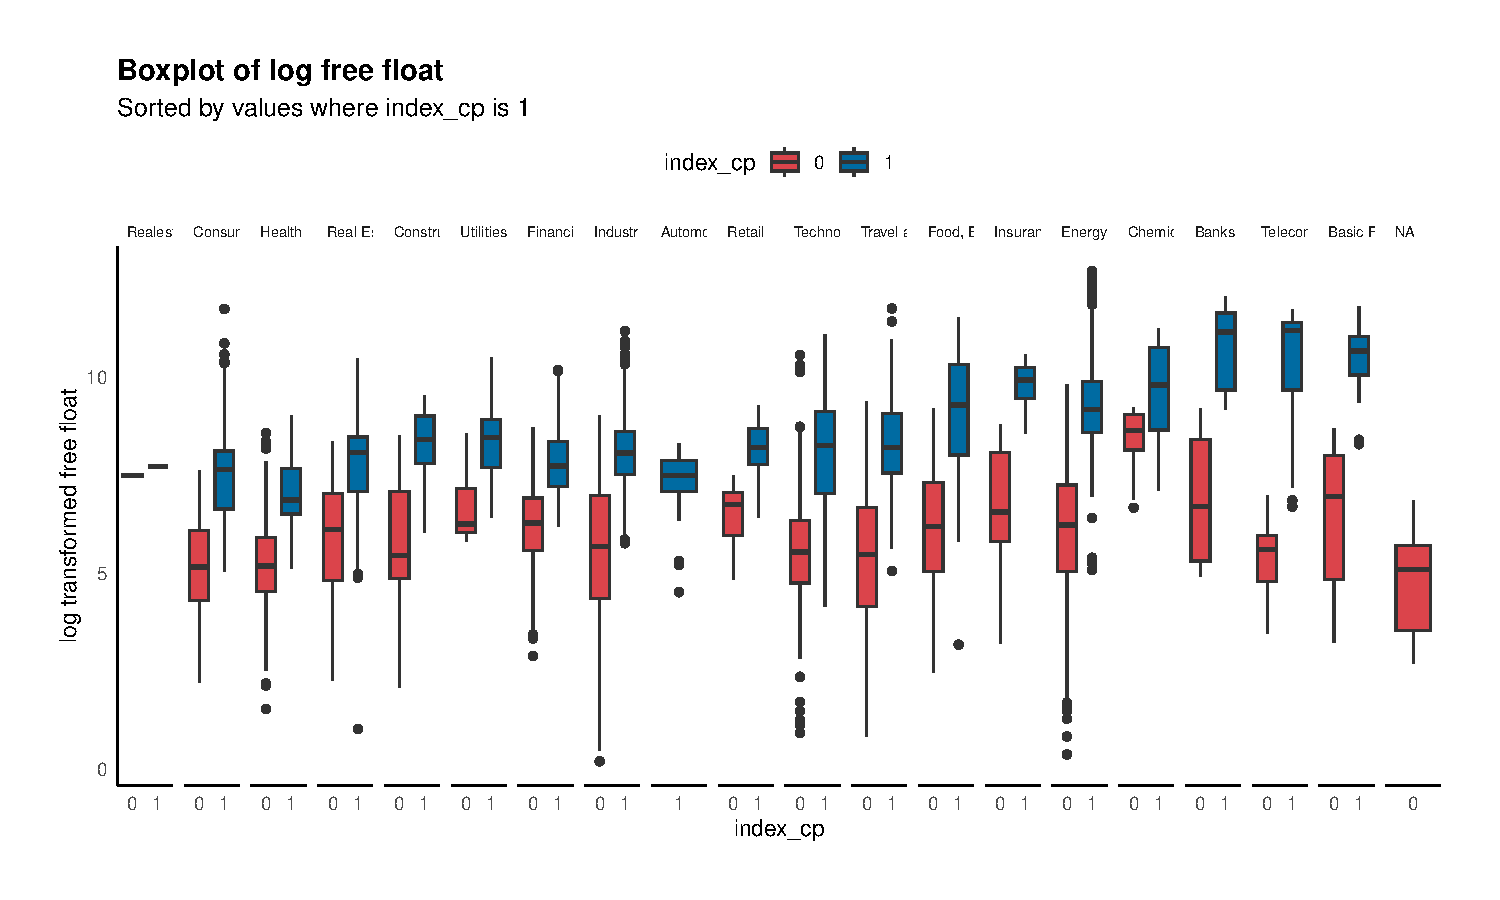
\includegraphics[width=\textwidth]{images/box_free_float.pdf}
    \caption{Box-plot \texttt{free\_float} and \texttt{index\_cp}}
    \subcaption*{Illustration of allocation of \texttt{index\_cp} per different ICB supersector, in relation to the logarithm of \texttt{free\_float}.}
    \label{fig:box_free_float}
\end{figure}

\begin{figure}[H]
    \centering
    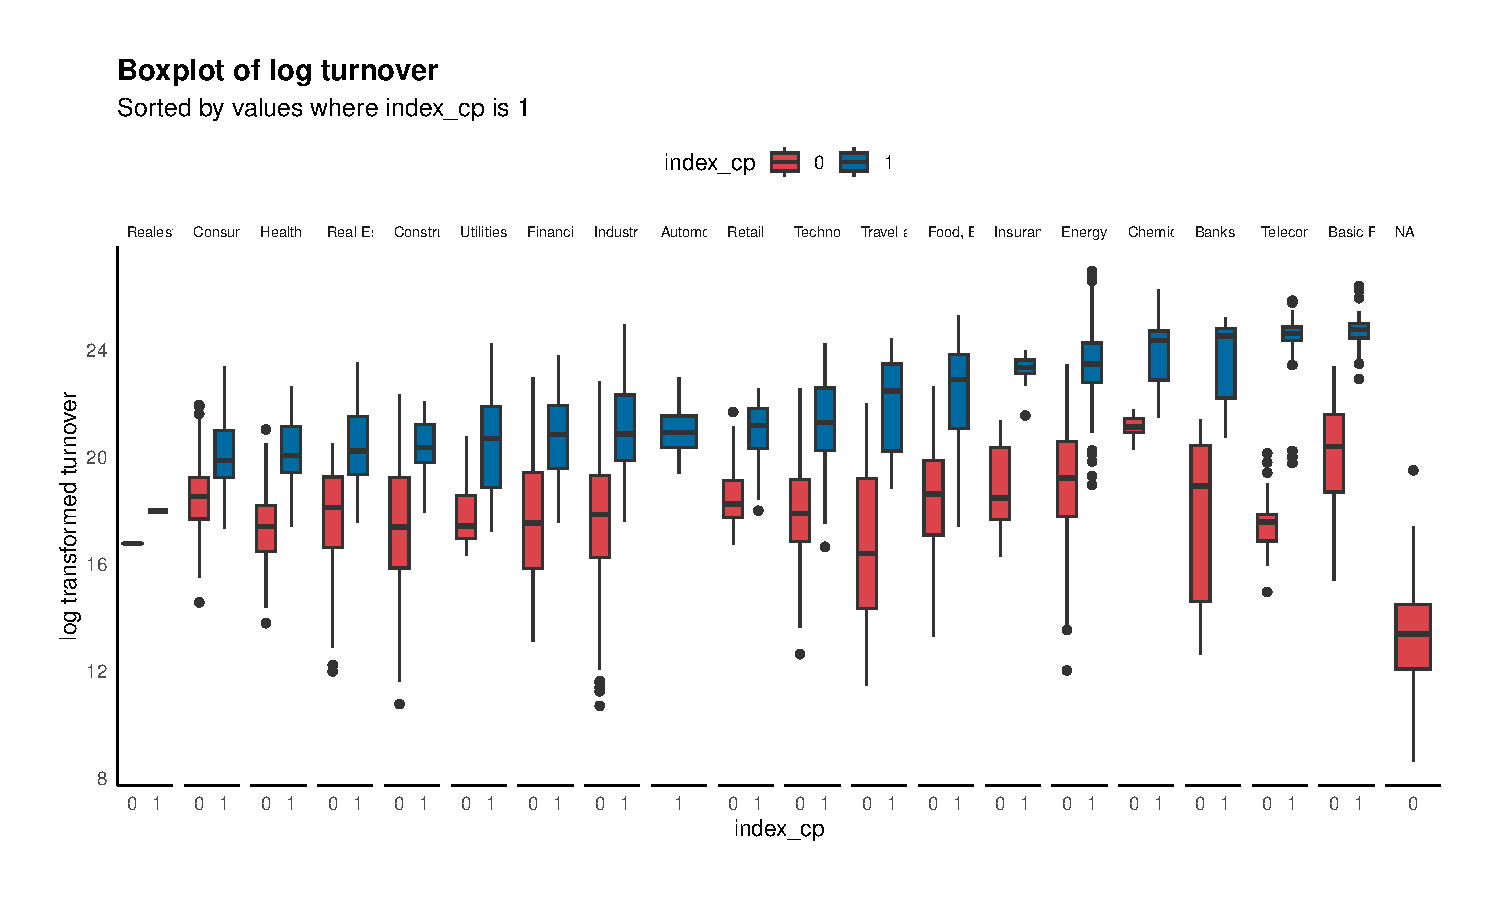
\includegraphics[width=\textwidth]{images/box_turnover.pdf}
    \caption{Box-plot \texttt{turnover\_eob} and \texttt{index\_cp}}
        \subcaption*{Illustration of allocation of \texttt{index\_cp} per different ICB supersector, in relation to the logarithm of \texttt{turnover\_eob}.}
    \label{fig:box_turnover}
\end{figure}

\begin{figure}[H]
    \centering
    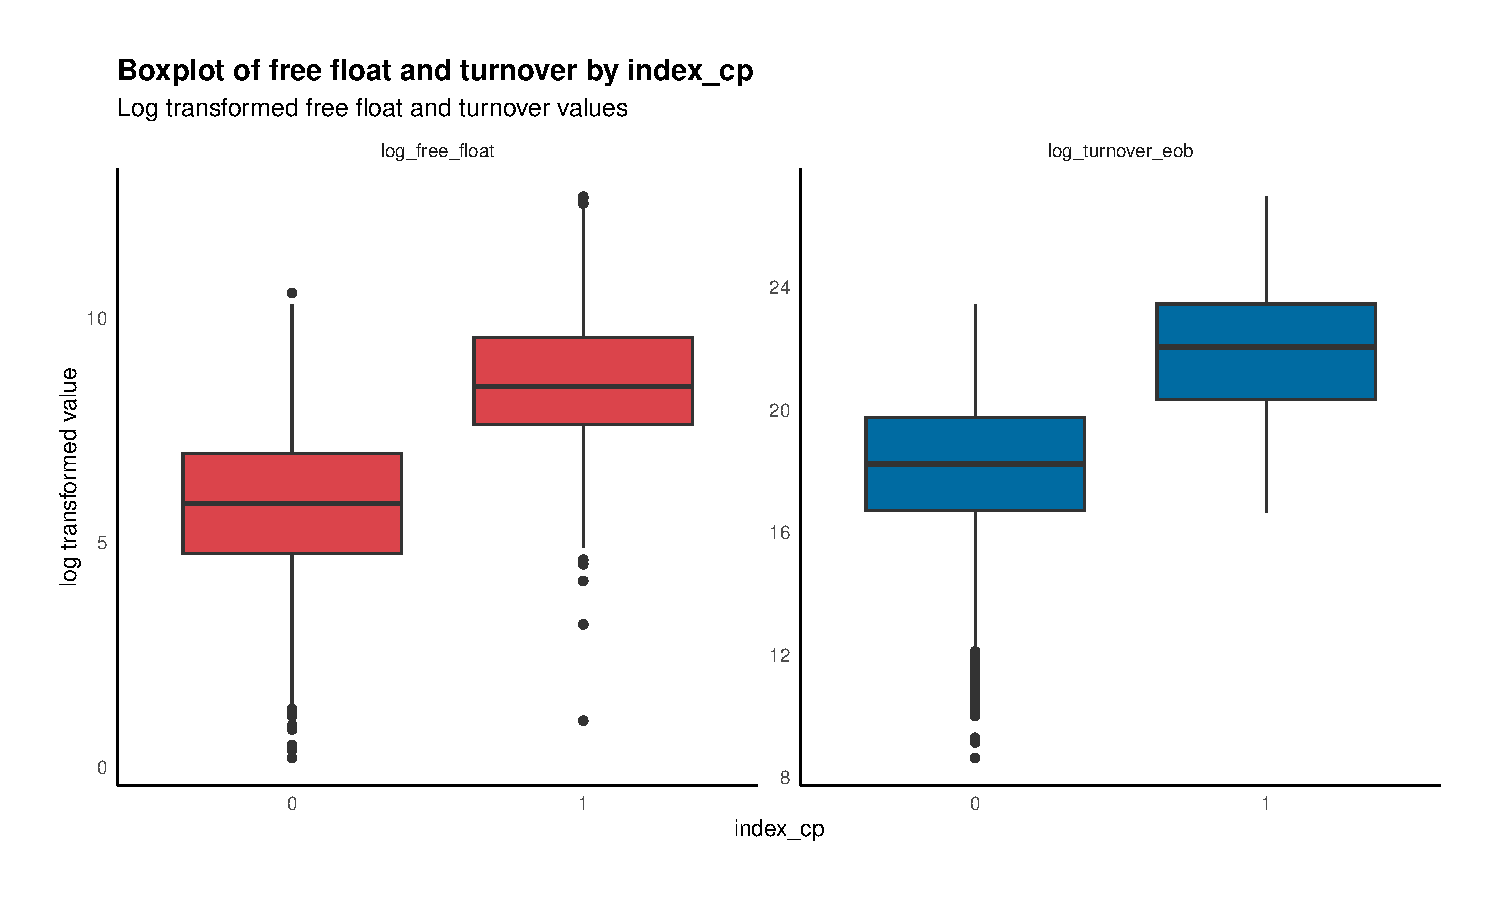
\includegraphics[width=\textwidth]{images/box_facetted.pdf}
    \caption{Box-plot \texttt{turnover\_eob}, \texttt{free\_float}, and \texttt{index\_cp}}
        \subcaption*{Boxplot of \texttt{free\_float} and \texttt{index\_cp}, and \texttt{turnover\_eob} and \texttt{index\_cp} }
    \label{fig:box_facetted}
\end{figure}


\begin{figure}[H]
    \centering
    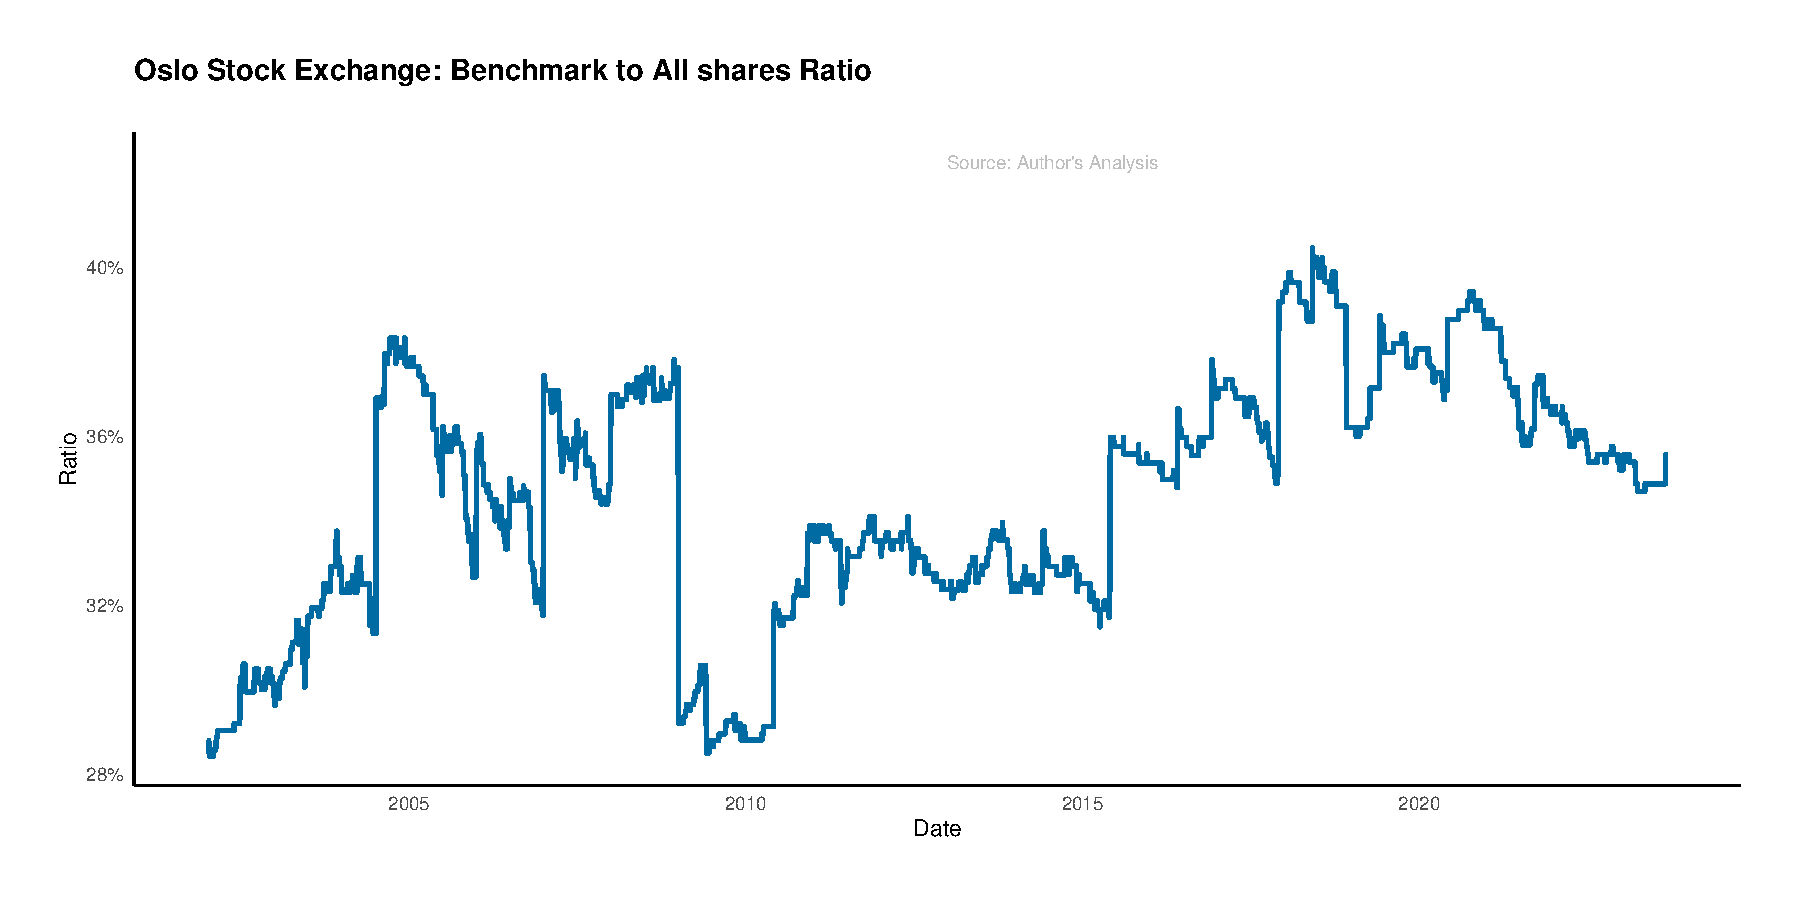
\includegraphics[width=\textwidth]{images/plot_share_126.pdf}
    \caption{Ratio of OSEBX to OSEAX member count}
    \label{Share of Benchmark to All shares over time}
\end{figure}

\begin{figure}[H]
    \centering
    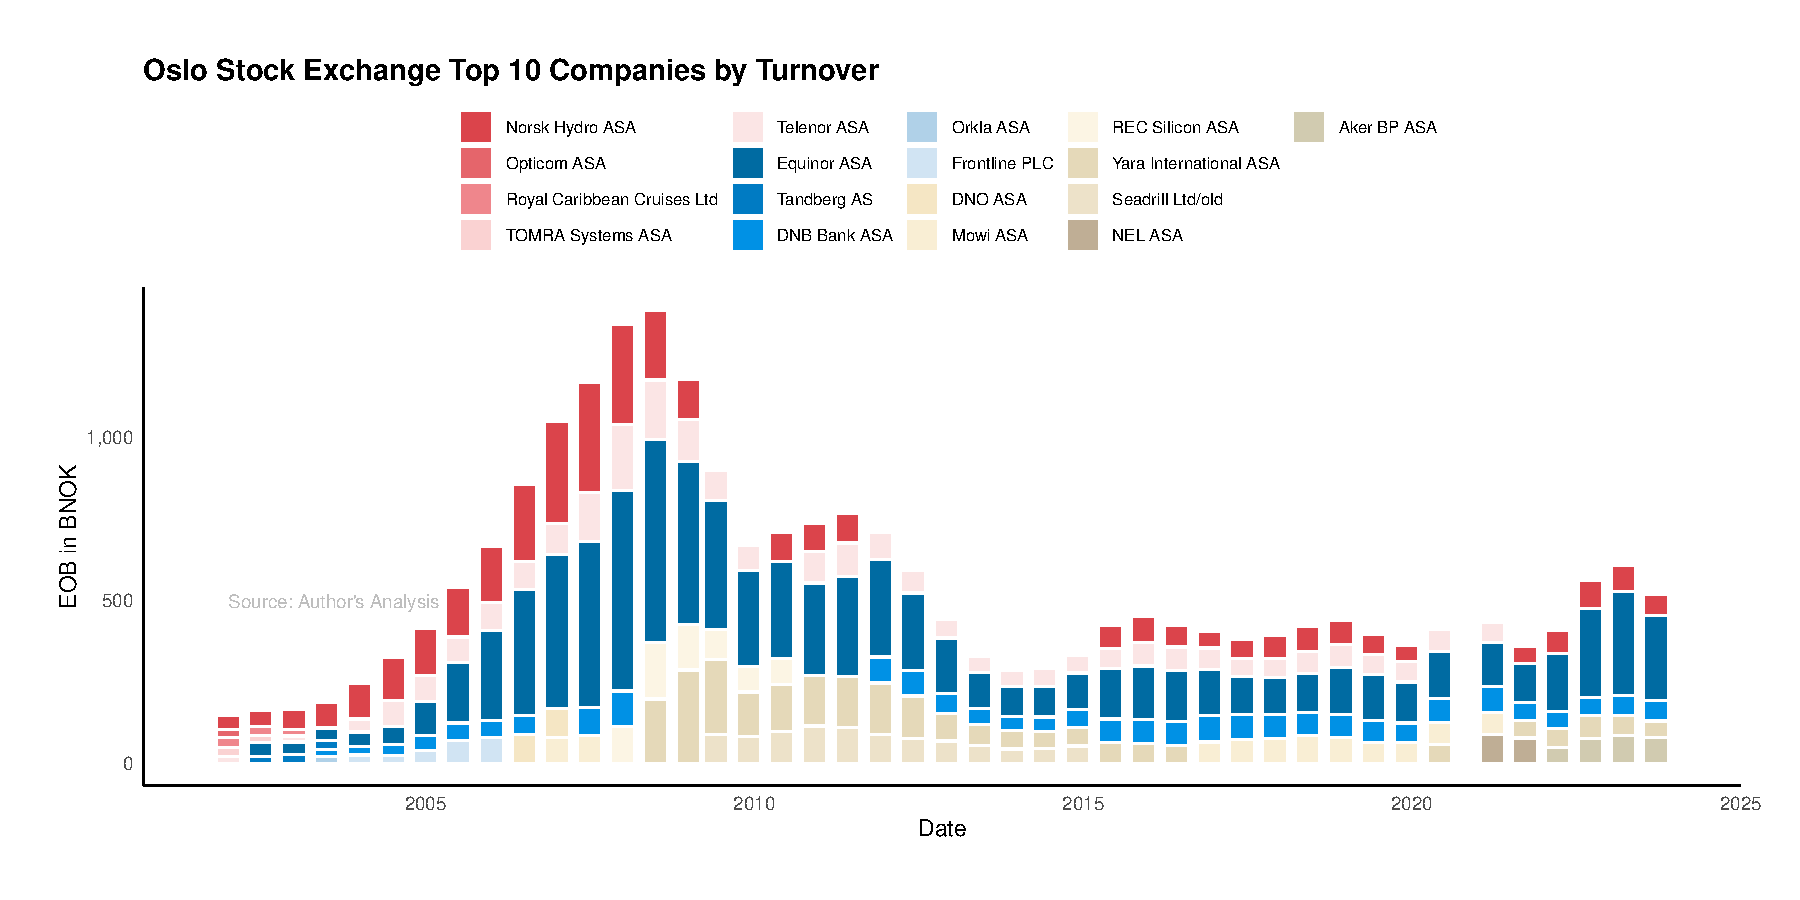
\includegraphics[width=\textwidth]{images/plot_turnover.pdf}
    \caption{Turnover of 10 largest OSEBX companies over time}
    \subcaption*{Turnover of 10 largest OSEBX companies over time, being large Norwegian Companies.}
    \label{OSEBX-top-10-turnover}
\end{figure}

\begin{figure}[H]
    \centering
    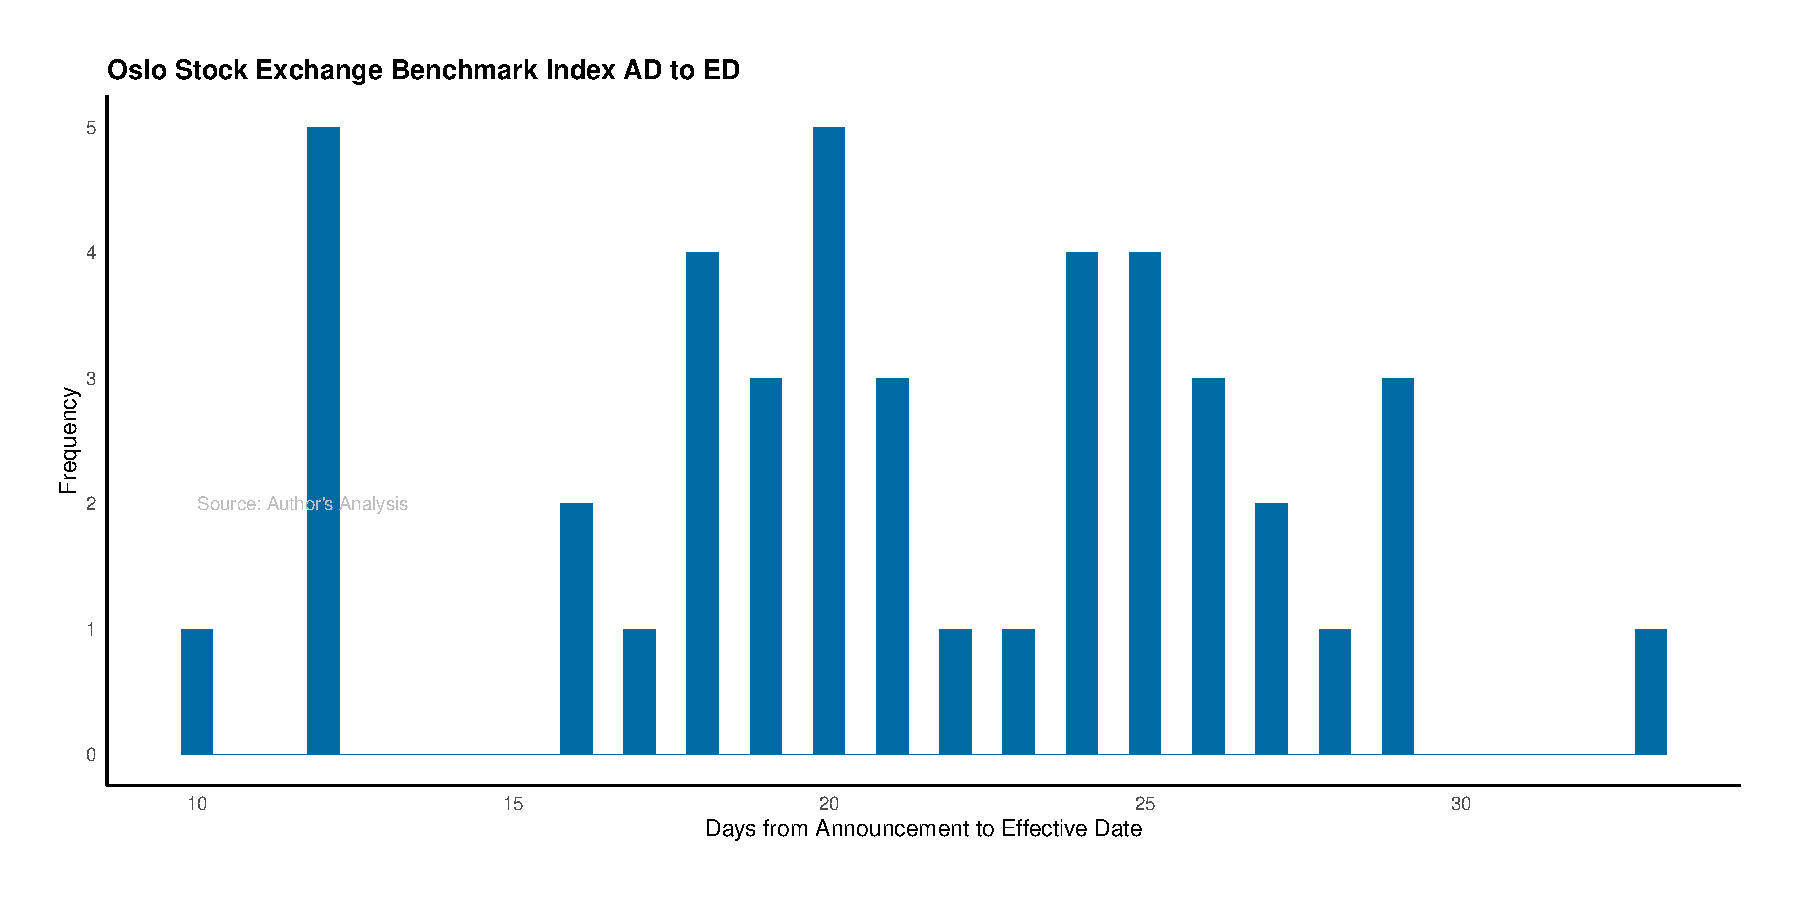
\includegraphics[width=\textwidth]{images/plot_ad_to_ed.pdf}
    \caption{OSEBX number of days from AD to ED}
        \subcaption*{Number of days between each announcement date and effective date illustrated as a histogram. The length varies between 10 and 32 days.}
    \label{OSEBX-ad-to-ed}
\end{figure}

\begin{figure}[H]
    \centering
    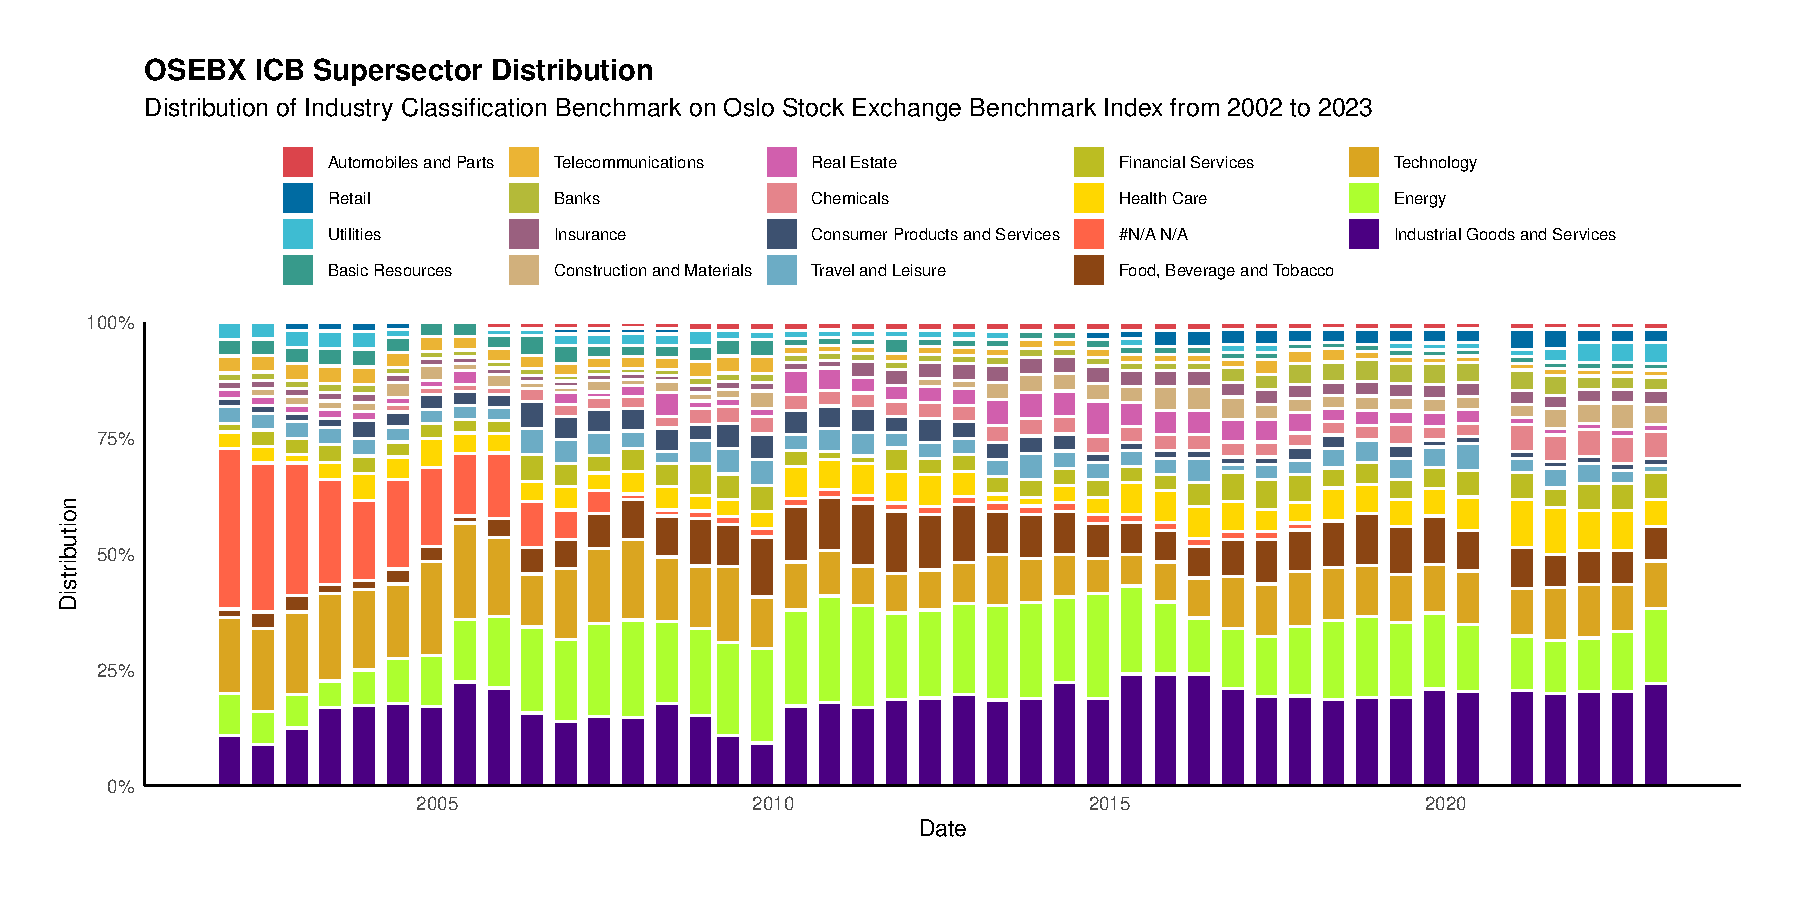
\includegraphics[width=0.9\textwidth]{images/plot_sectors.pdf}
    \caption{{OSEBX ICB Supersector Distribution over Time}}
    \subcaption*{Industry classification benchmark (ICB) for companies on OSEBX in the period from 2002 to 2023. Notice that industry and energy companies dominate OSEBX.}
    \label{Oslo Stock Exchange Benchmark Index Sector Distribution}
\end{figure}

% \begin{figure}[H]
%     \centering
%     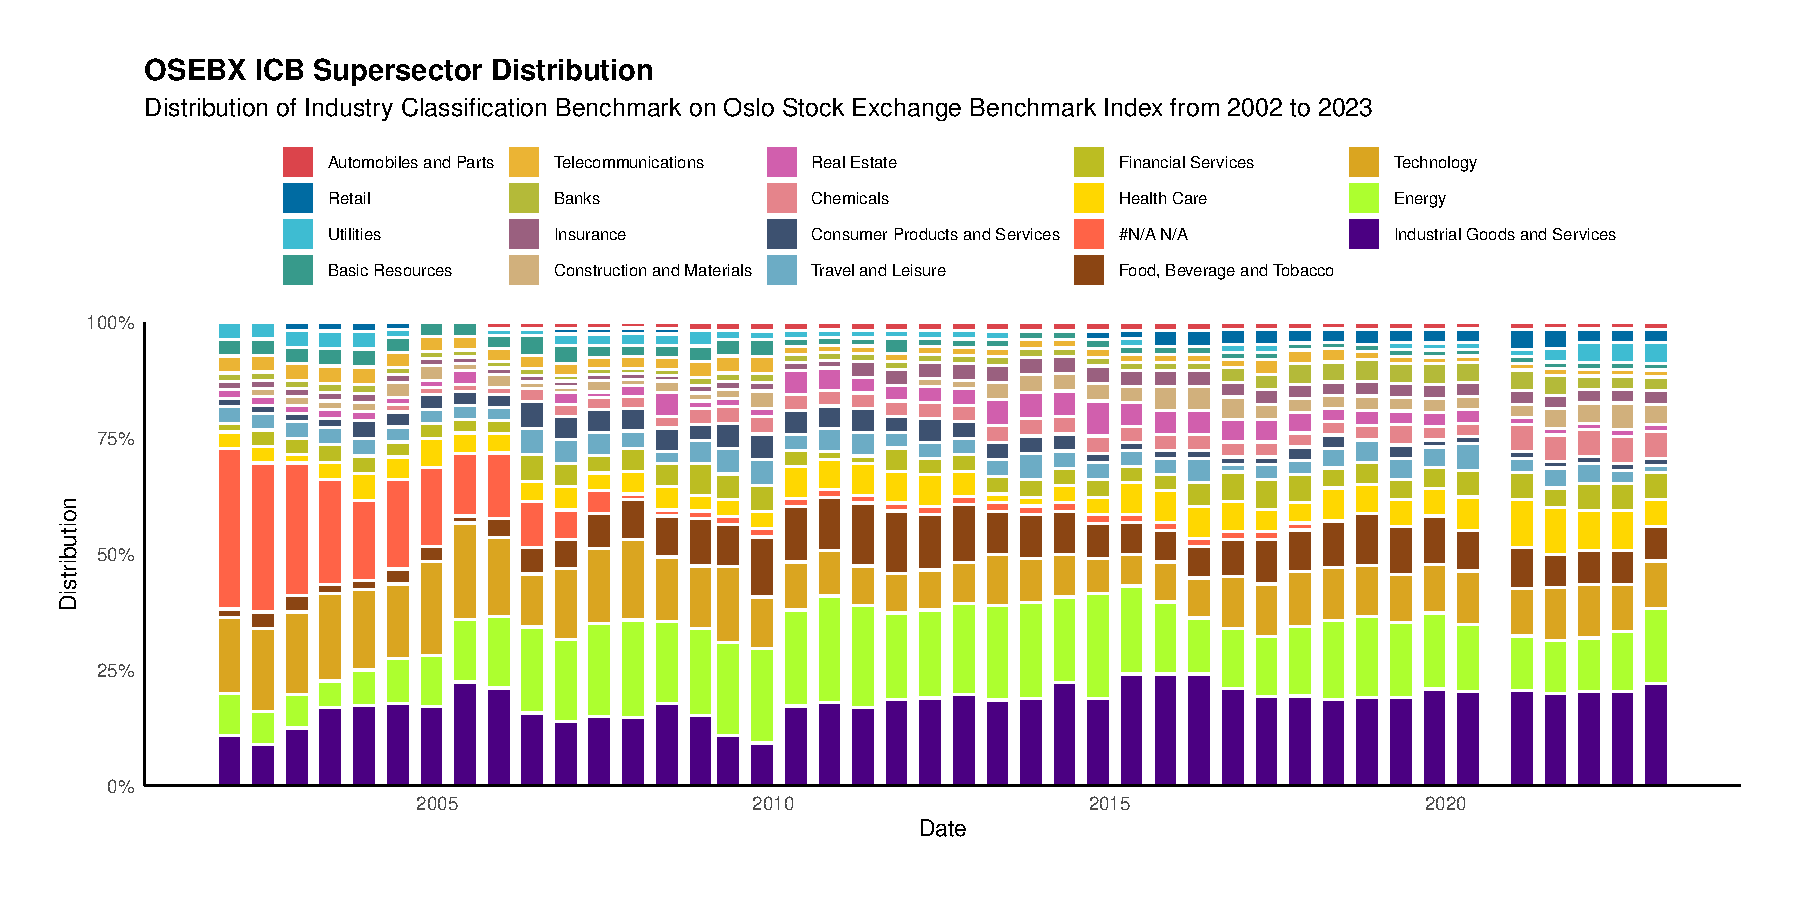
\includegraphics[width=\textwidth]{images/plot_sectors.pdf}
%     \caption{Oslo Stock Exchange Benchmark Index Sector Distribution}
%     \label{Oslo Stock Exchange Benchmark Index Sector Distribution}
% \end{figure}

% \begin{figure}[H]
%     \centering
%     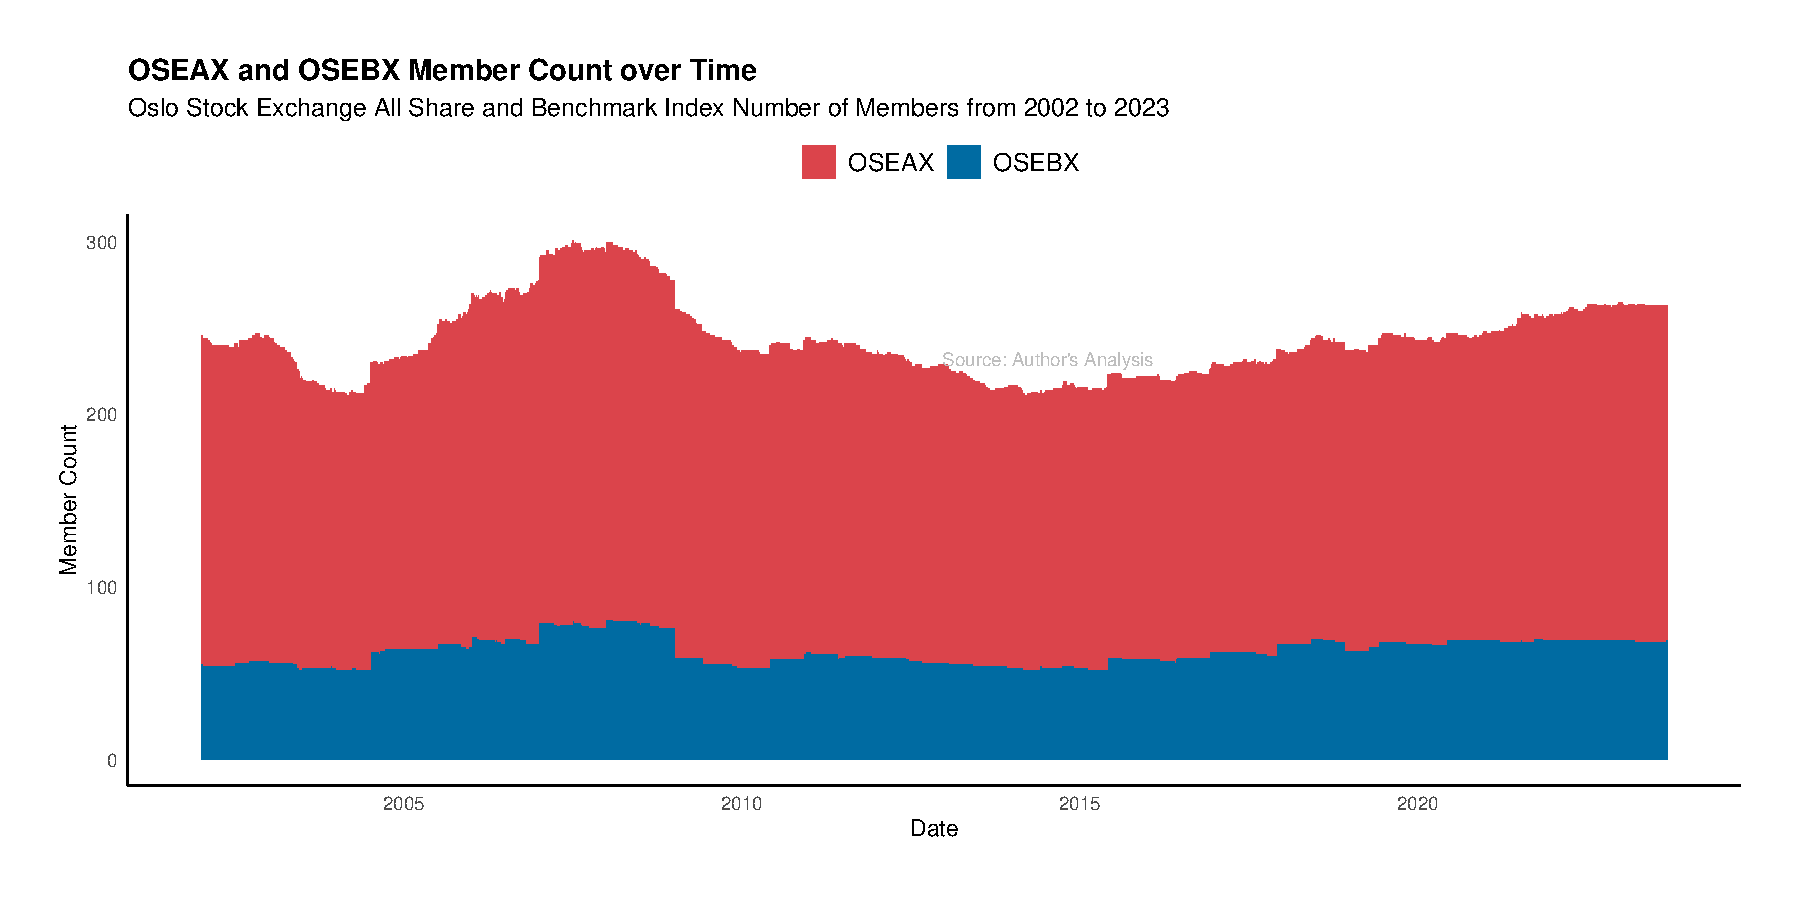
\includegraphics[width=\textwidth]{images/plot_memb_126.pdf}
%     \caption{Members over time}
%     \label{Members over time}
% \end{figure}



% Portfolios

\begin{figure}[H]
    \centering
    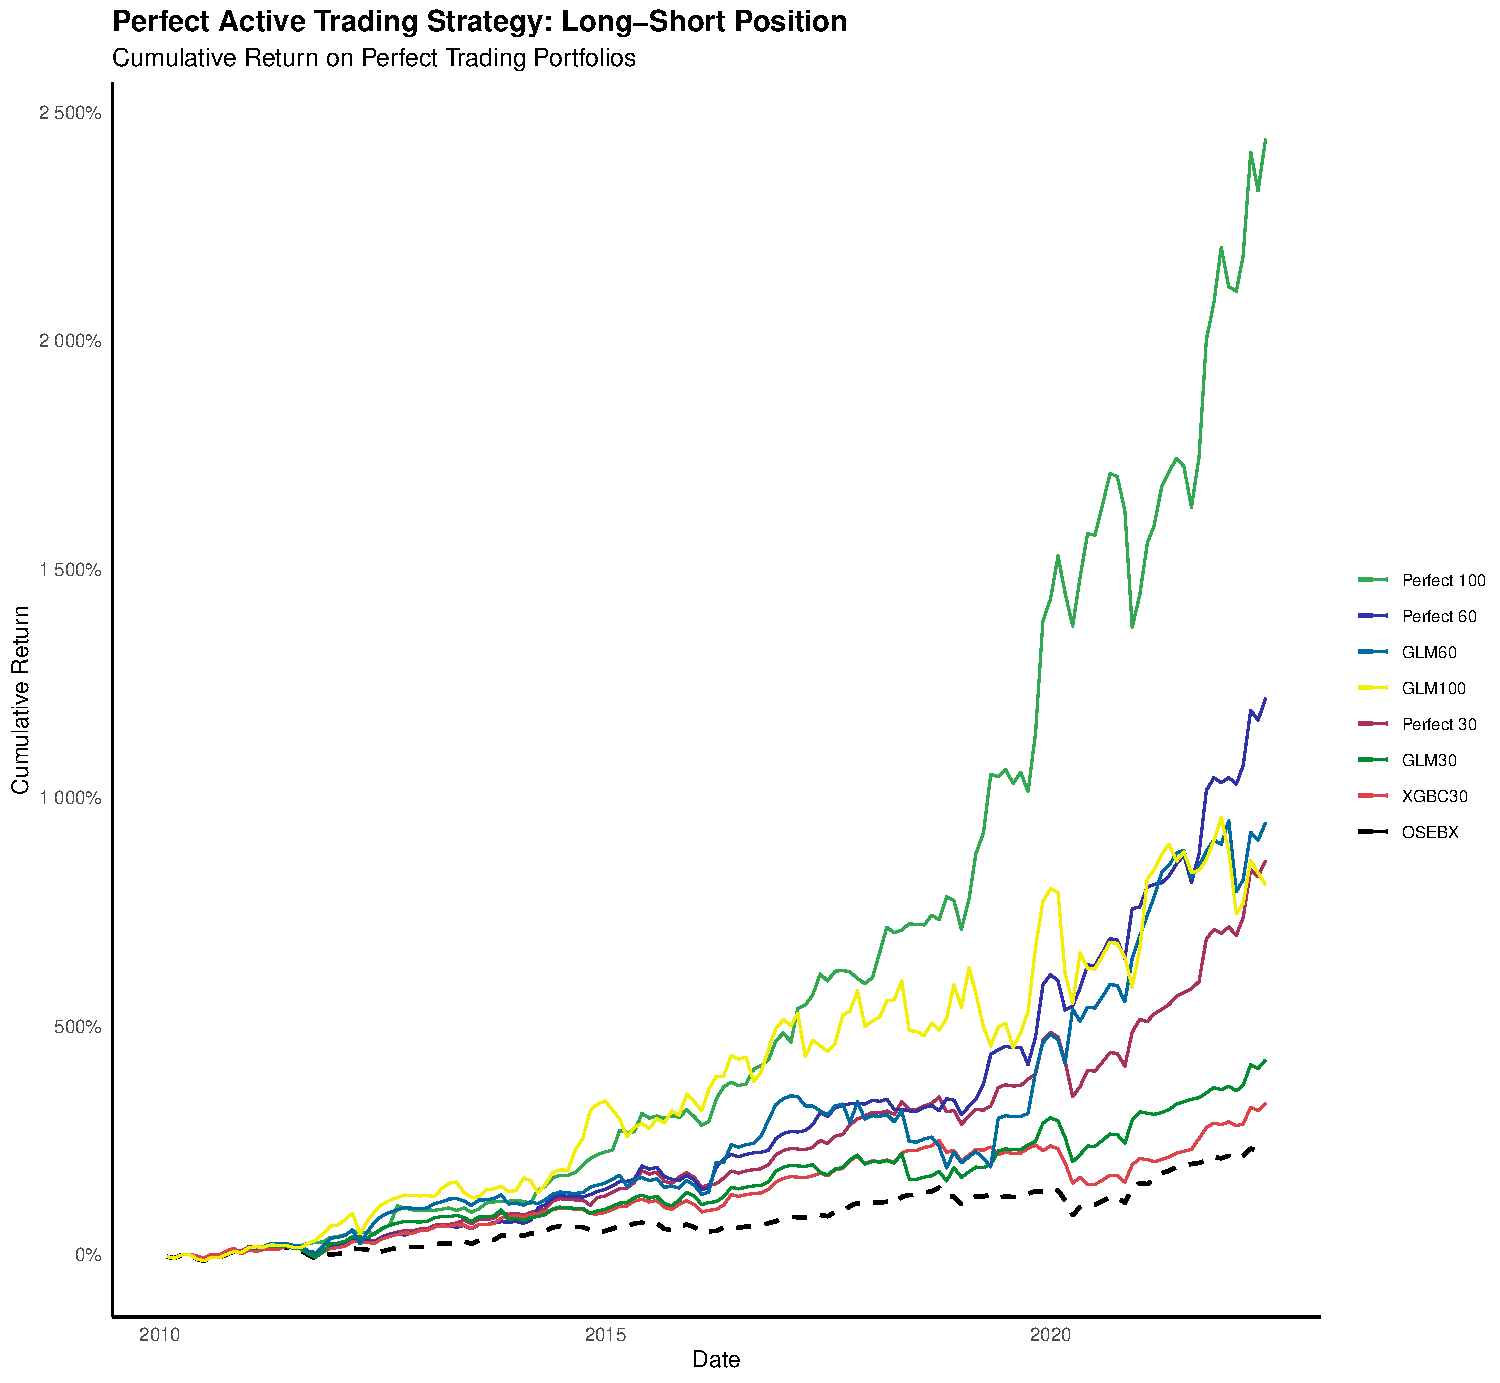
\includegraphics{images/perfect_port_monthly.pdf}
    % \vspace{1em}
    \caption{Cumulative Return Perfect Portolios}
    \subcaption*{In this figure we have included the portfolios Perfect 30, Perfect 60, and Perfect 100. Those portfolios represent the development if one had known 100\% of which companies should enter/exit OSEBX since 2010. Investing NOK 1000 on January 4th, 2010 would have grown to 25,000 on May 31st, 2022, if one knew the changes 100 days in advance of the ED, beating OSEBX by thousands of percent in cumulative return. }
    \label{fig:trading-perfect}
\end{figure}

\newpage

\begin{figure}[H]
    \centering
    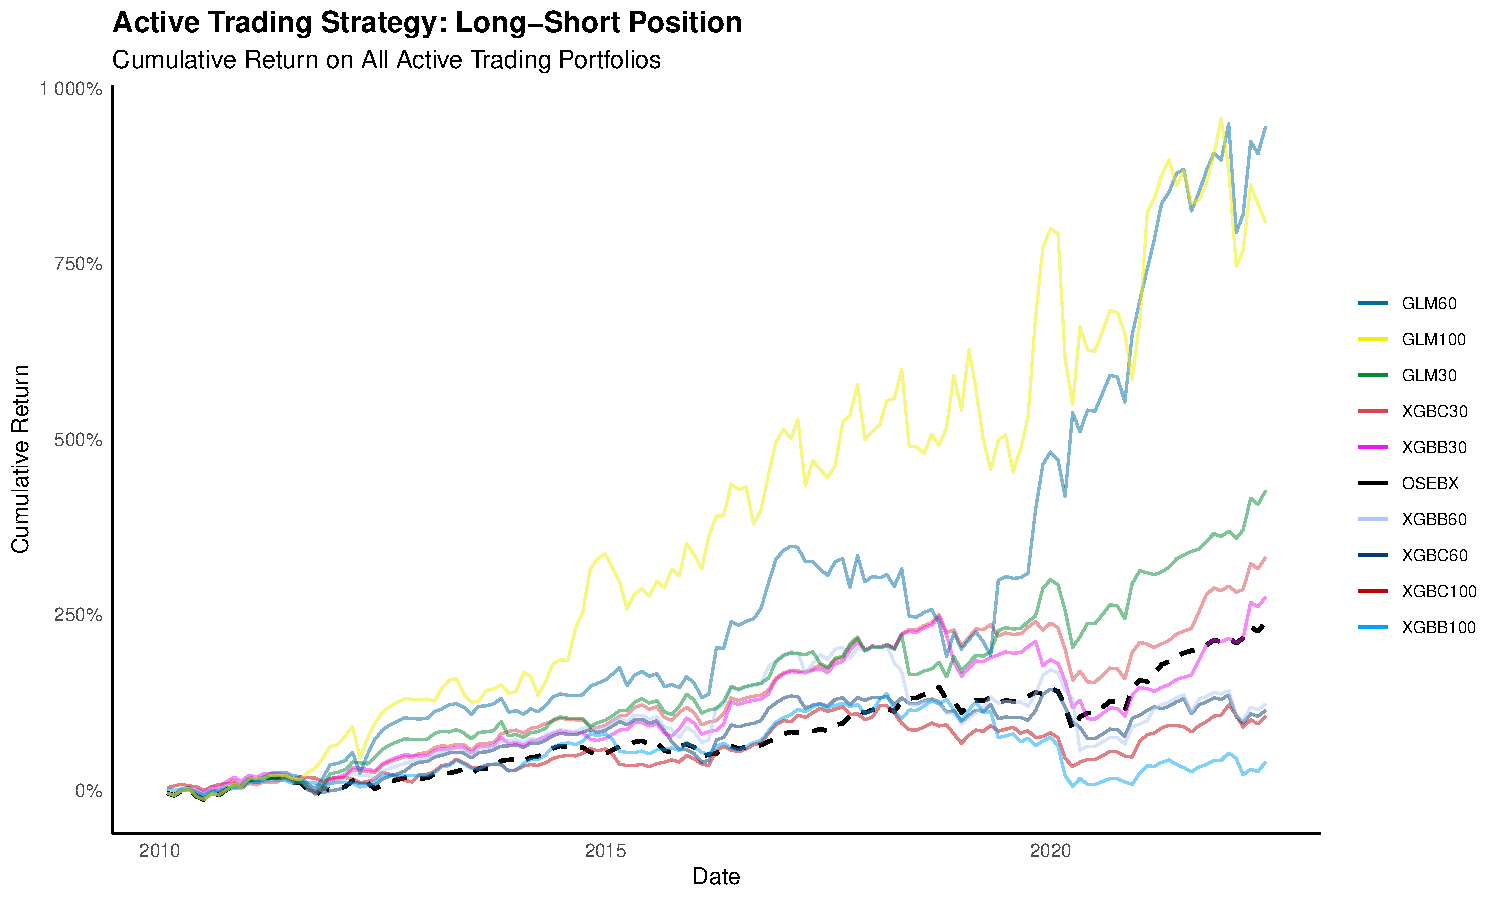
\includegraphics{images/trading_long_short_all.pdf}
    % \vspace{1em}
    \caption{Cumulative Return Long-Short Trading Strategy}
        \subcaption*{All long-short portfolios simulated are illustrated. }
    \label{fig:long-short-all}
\end{figure}

\begin{figure}[H]
    \centering
    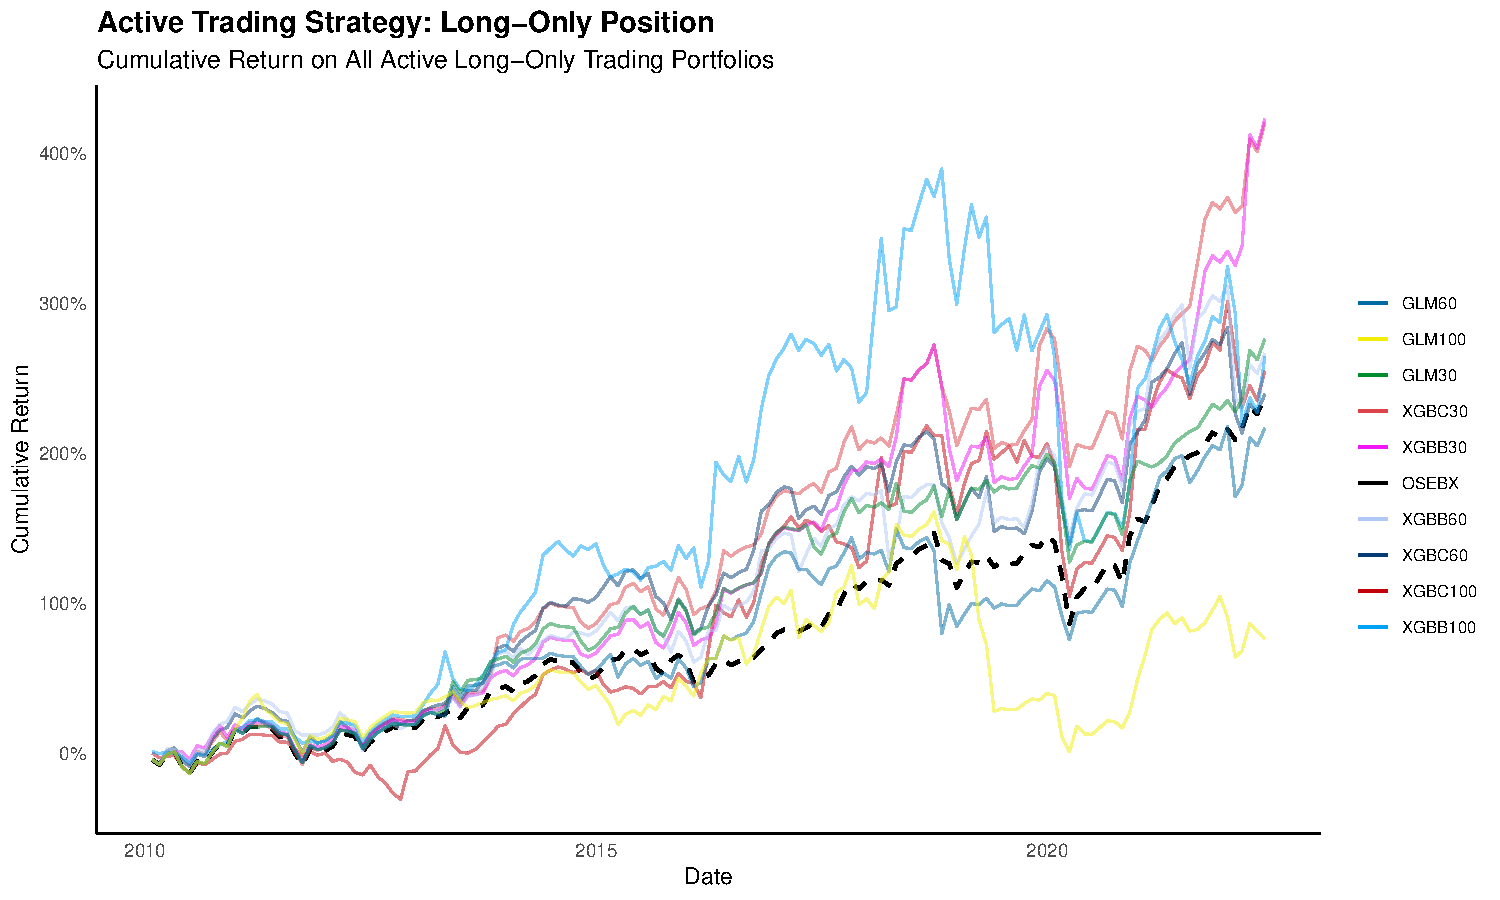
\includegraphics{images/trading_long_only_all.pdf}
    % \vspace{1em}
    \caption{Cumulative Return Long-Only Trading Strategy}
            \subcaption*{All long-only portfolios simulated are illustrated. }
    \label{fig:long-only-all}
\end{figure}

\begin{figure}[H]
    \centering
    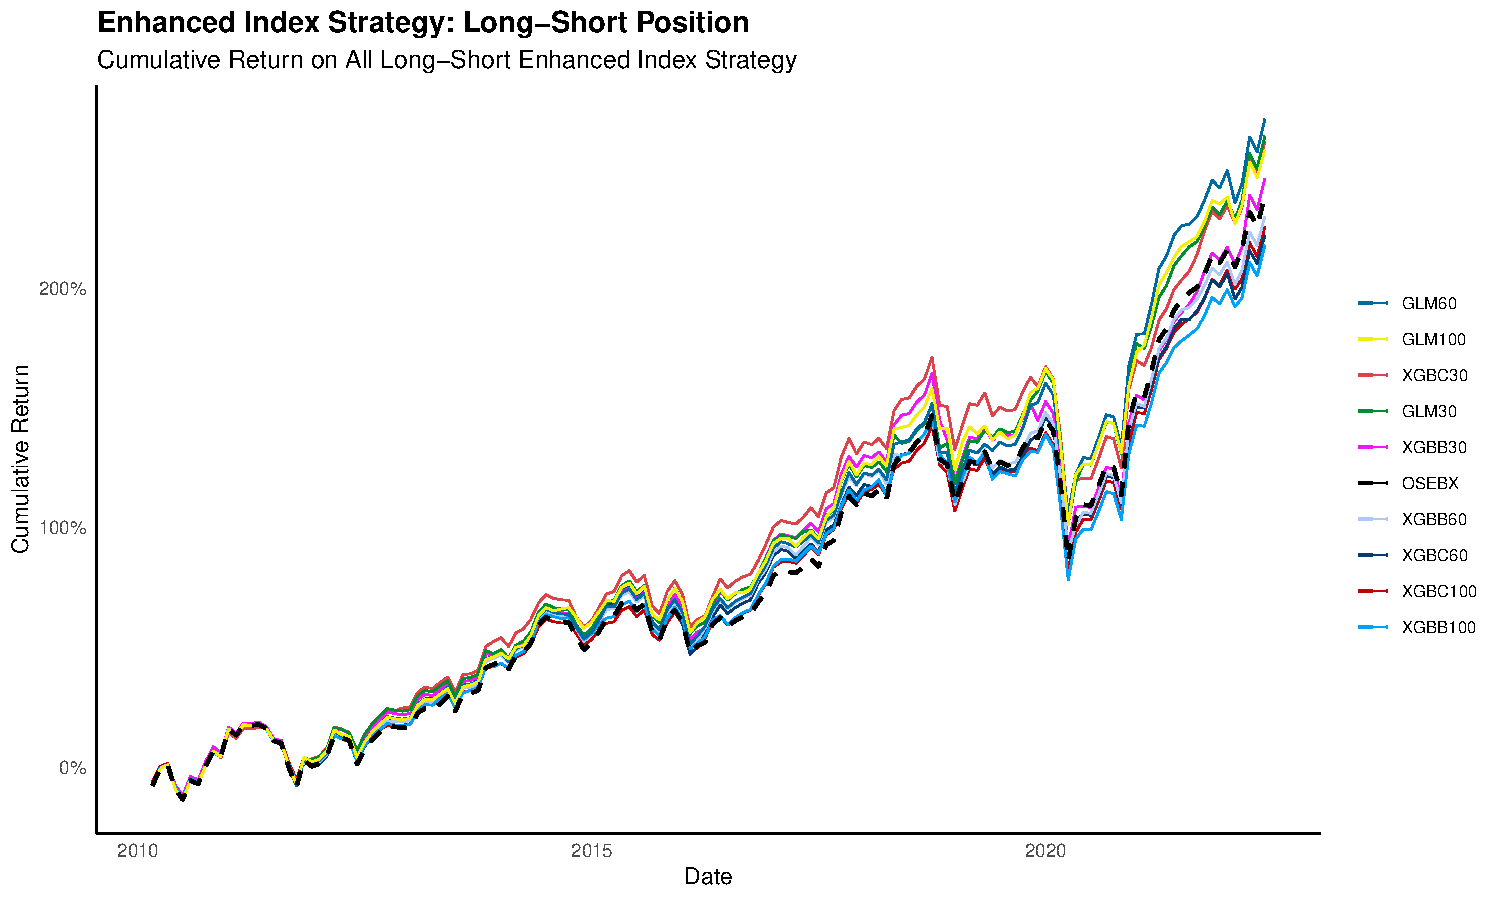
\includegraphics{images/enhanced_long_short_all.pdf}
    \caption{Cumulative Return Long-Short Enhanced Index}
            \subcaption*{All long-short enhanced portfolios simulated are illustrated. }
    \label{fig:enhanced-long-only-all}
\end{figure}

\begin{figure}[H]
    \centering
    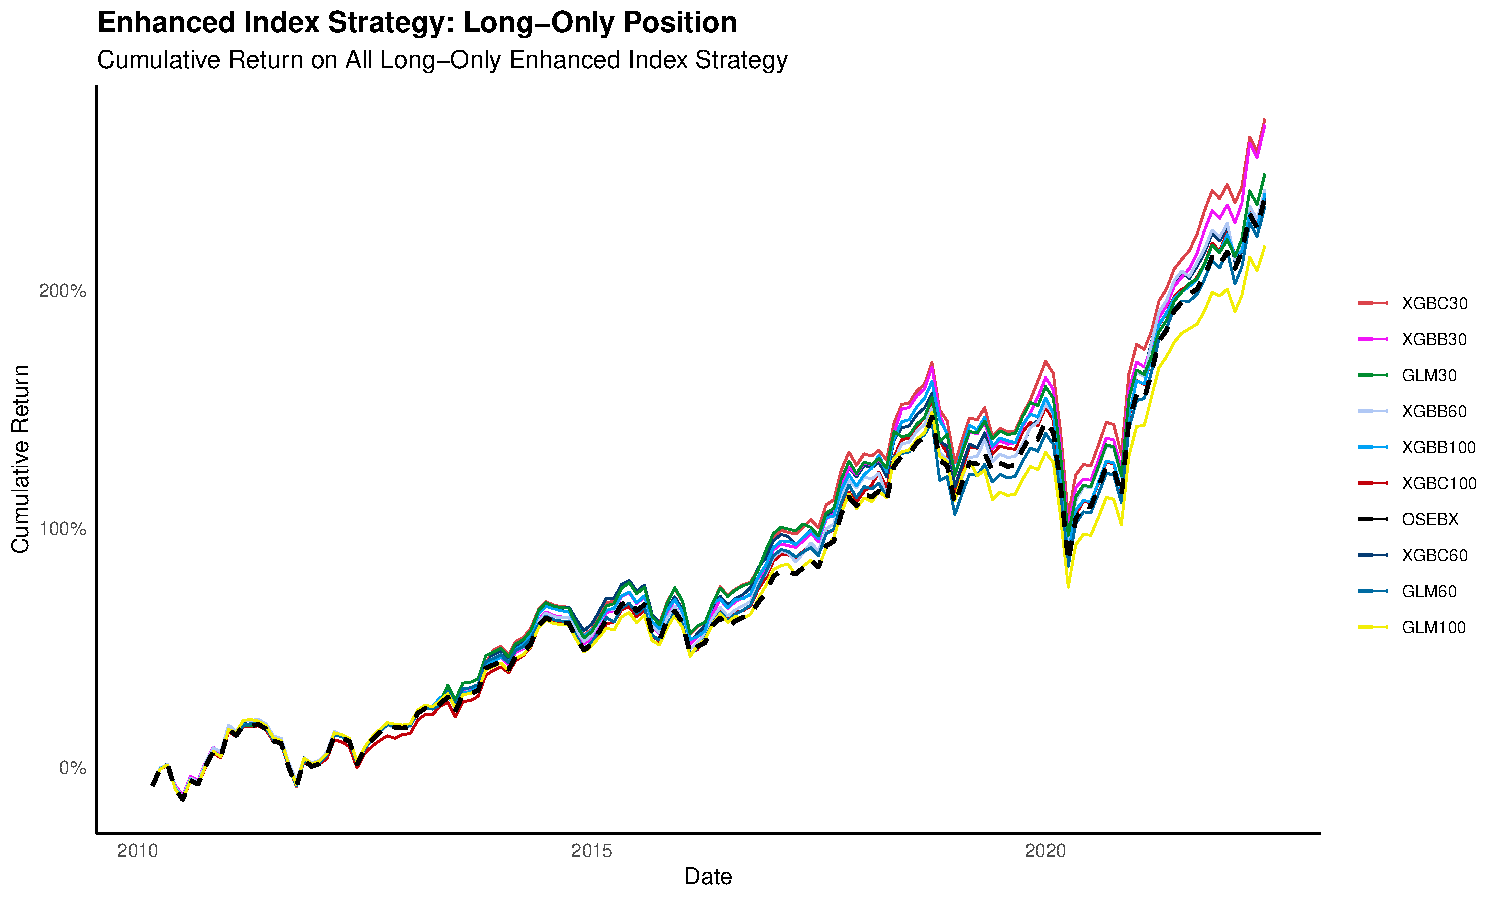
\includegraphics{images/enhanced_long_only_all.pdf}
    \caption{Cumulative Return Long-Only Enhanced Index}
                \subcaption*{All long-only enhanced portfolios simulated are illustrated. }
    \label{fig:enhanced-long-short-all}
\end{figure}
\newpage
\section{Portfolio Simulation Algorithm}
\label{APPENDIX Portfolio Simulation Algorithm}

The algorithm used when performing the portfolio simulations can be summarised as the following. All predictions come from the ML models, which are stored in a data frame including the dates of the start and end of the trading periods, and which companies are held in each trading period.

\textbf{Step 1:} Add OSEBX as a long position between each active trading period.

\textbf{Step 2:} Find VWAP for each company for each trading period start and end date, including all periods OSEBX is traded.

\textbf{Step 3:} Remove any rows with NA-values in VWAP (most present for companies in 2010 and 2011).

\textbf{Step 4:} Calculate the return on each trade, illustrated in \autoref{return_explaination_app} where $r_l$ is the return on a long position, $r_l$ is the return on short positions, $p_0$ is the VWAP at the start of the trading period and $p_1$ is the VWAP at the end of the trading period. $S_{rate}$ is the annual short rate, and $d$ is the number of days per active trading period (30, 60, or 100 days). 
\begin{equation}
\begin{aligned}
    r_l = \frac{p_1 - p_0 }{p_0} &  ,  &r_s = \frac{p_0 - p_1 }{p_0}-\frac{S_{rate}^{ann}*d}{365} 
\label{return_explaination_app}
\end{aligned}
\end{equation}

\textbf{Step 5:} Calculate the average return for each trading period, as we assume weights between the assets to be equally weighted.

\textbf{Step 6:} Define an amount of money to start with (we used 10 million). For each trading period, multiply the money at the end of the last period by the average return in that period plus 1, minus 8 bps (as we use 4 bps as transaction cost per trade, but at the end of each period we both sell the previous holdings and buy new holdings, therefore 8 bps). 

\newpage
\section{Example of Portfolio Simulation}
\label{APPENDIX Portfolio Simulation of GLM100-portfolio}
We decided to include the GLM100 portfolio as an example of a simulated portfolio. Please note that this simulation only yields portfolio size at the end of the trading periods, so in practice, we have calculated the return for each day and extracted the return from the same dates as the FF3 factors are reported (being the last date in each month). The point of this Appendix is to illustrate where the exceptional (yet risky) returns come from. 

\begin{table}[h]
\centering
\scriptsize
\begin{tabular}{llllllrrr}
  \hline
Start & End & Company & $Y_{i,t}$ & $\widehat Y_{i,t}$ & $Y_{i,t-1}$ & VWAP start & VWAP end & Return \\ 
\hline
   2010-01-04 & 2011-01-08 & OSEBX &  &  &  & 380.15 & 439.92 & 0.16 \\ 
   2011-01-11 & 2011-05-31 & AKER NO Equity & 0 & 1 & 0 & 141.72 & 153.58 & 0.08 \\ 
   2011-01-11 & 2011-05-31 & ELT NO Equity & 1 & 0 & 1 & 1.00 & 1.00 & -0.01 \\ 
   2011-01-11 & 2011-05-31 & JIN NO Equity & 0 & 0 & 1 & 19.86 & 16.40 & 0.16 \\ 
   2011-01-11 & 2011-05-31 & QFR NO Equity & 1 & 0 & 1 & 16.90 & 17.87 & -0.07 \\ 
   2011-06-01 & 2011-07-10 & OSEBX &  &  &  & 437.39 & 421.46 & -0.04 \\ 
   2011-07-13 & 2011-11-30 & MGN NO Equity & 1 & 0 & 1 & 11.21 & 5.14 & 0.53 \\ 
   2011-07-13 & 2011-11-30 & QEC NO Equity & 0 & 0 & 1 & 5.56 & 3.97 & 0.28 \\ 
   2011-12-01 & 2012-01-09 & OSEBX &  &  &  & 378.59 & 389.09 & 0.03 \\ 
   2012-01-12 & 2012-05-31 & MGN NO Equity & 0 & 0 & 1 & 6.41 & 5.21 & 0.18 \\ 
   2012-06-01 & 2013-01-08 & OSEBX & &  &  & 377.66 & 456.04 & 0.21 \\ 
   2013-01-11 & 2013-05-31 & EMGS NO Equity & 1 & 0 & 1 & 214.05 & 208.01 & 0.02 \\ 
   2013-01-11 & 2013-05-31 & SONG NO Equity & 0 & 0 & 1 & 1.00 & 1.00 & -0.01 \\ 
   2013-06-01 & 2013-07-09 & OSEBX &  &  &  & 491.71 & 482.30 & -0.02 \\ 
   2013-07-12 & 2013-11-29 & BRG NO Equity & 0 & 1 & 0 & 26.89 & 26.65 & -0.01 \\ 
   2013-07-12 & 2013-11-29 & AFG NO Equity & 1 & 0 & 1 & 61.82 & 68.07 & -0.11 \\ 
   2013-07-12 & 2013-11-29 & EMGS NO Equity & 0 & 0 & 1 & 198.11 & 157.16 & 0.20 \\ 
   2013-07-12 & 2013-11-29 & PLCS NO Equity & 1 & 0 & 1 & 432.09 & 409.77 & 0.04 \\ 
   2013-11-30 & 2014-01-07 & OSEBX &  &  &  & 542.79 & 547.04 & 0.01 \\ 
   2014-01-10 & 2014-05-30 & PLCS NO Equity & 0 & 0 & 1 & 417.46 & 341.25 & 0.17 \\ 
   2014-05-31 & 2014-07-08 & OSEBX &  &  &  & 605.26 & 619.53 & 0.02 \\ 
   2014-07-11 & 2014-11-28 & ASTK NO Equity & 0 & 0 & 1 & 18.94 & 9.14 & 0.51 \\ 
   2014-11-29 & 2015-01-06 & OSEBX &  &  &  & 566.34 & 569.98 & 0.01 \\ 
   2015-01-09 & 2015-05-29 & LSG NO Equity & 0 & 1 & 0 & 28.18 & 25.26 & -0.10 \\ 
   2015-05-30 & 2015-07-10 & OSEBX &  &  &  & 645.68 & 634.87 & -0.02 \\ 
   2015-07-13 & 2015-11-30 & LSG NO Equity & 0 & 1 & 0 & 27.35 & 31.87 & 0.17 \\ 
   2015-07-13 & 2015-11-30 & SCHB NO Equity & 1 & 1 & 0 & 184.81 & 223.98 & 0.21 \\ 
   2015-12-01 & 2016-01-09 & OSEBX &  &  &  & 632.46 & 563.75 & -0.11 \\ 
   2016-01-12 & 2016-05-31 & LSG NO Equity & 0 & 1 & 0 & 31.95 & 42.64 & 0.33 \\ 
   2016-06-01 & 2016-07-10 & OSEBX &  &  &  & 611.63 & 610.32 & -0.00 \\ 
   2016-07-13 & 2016-11-30 & AUSS NO Equity & 0 & 1 & 0 & 73.86 & 80.46 & 0.09 \\ 
   2016-07-13 & 2016-11-30 & LSG NO Equity & 1 & 1 & 0 & 41.26 & 47.08 & 0.14 \\ 
   2016-12-01 & 2017-01-08 & OSEBX &  &  &  & 662.79 & 694.57 & 0.05 \\ 
   2017-01-11 & 2017-05-31 & AUSS NO Equity & 0 & 1 & 0 & 77.41 & 71.05 & -0.08 \\ 
   2017-01-11 & 2017-05-31 & GSF NO Equity & 1 & 1 & 0 & 72.68 & 63.21 & -0.13 \\ 
   2017-06-01 & 2017-07-10 & OSEBX &  &  &  & 713.19 & 702.25 & -0.02 \\ 
   2017-07-13 & 2017-11-30 & BANO NO Equity & 1 & 1 & 0 & 81.12 & 95.05 & 0.17 \\ 
   2017-07-13 & 2017-11-30 & AUSS NO Equity & 0 & 1 & 0 & 68.92 & 70.13 & 0.02 \\ 
   2017-12-01 & 2018-01-08 & OSEBX &  &  &  & 798.41 & 834.73 & 0.05 \\ 
   2018-01-11 & 2018-05-31 & QEC NO Equity & 1 & 0 & 1 & 6.11 & 5.70 & 0.06 \\ 

 
    \midrule \multicolumn{9}{r}{{Continued on next page}} \\
   \hline
\end{tabular}
   
\end{table}



\begin{table}[H]
\centering
\scriptsize
\begin{tabular}{llllllrrr}
 \midrule \multicolumn{9}{r}{{Continuation of previous page}} \\
  \hline
Start & End & Company & $Y_{i,t}$ & $\widehat Y_{i,t}$ & $Y_{i,t-1}$ & VWAP start & VWAP end & Return \\ 
  \hline 
   2018-01-11 & 2018-05-31 & 1643322D NO Equity & 0 & 0 & 1 & 581.85 & 952.72 & -0.65 \\ 
   2018-01-11 & 2018-05-31 & B2I NO Equity & 0 & 1 & 0 & 20.69 & 18.25 & -0.12 \\ 
   2018-01-11 & 2018-05-31 & AUSS NO Equity & 1 & 1 & 0 & 65.94 & 97.46 & 0.48 \\ 
   2018-06-01 & 2018-07-10 & OSEBX &  &  &  & 880.53 & 899.13 & 0.02 \\ 
   2018-07-13 & 2018-11-30 & QEC NO Equity & 0 & 0 & 1 & 3.05 & 2.56 & 0.15 \\ 
   2018-12-01 & 2019-01-08 & OSEBX &  &  &  & 860.98 & 836.40 & -0.03 \\ 
   2019-01-11 & 2019-05-31 & RECSI NO Equity & 1 & 0 & 1 & 6.57 & 4.93 & 0.24 \\ 
   2019-01-11 & 2019-05-31 & SASNO NO Equity & 0 & 1 & 0 & 5.86 & 3.22 & -0.45 \\ 
   2019-06-01 & 2019-07-09 & OSEBX &  &  &  & 852.09 & 883.18 & 0.04 \\ 
   2019-07-12 & 2019-11-29 & RECSI NO Equity & 0 & 0 & 1 & 4.67 & 2.68 & 0.42 \\ 
   2019-11-30 & 2020-01-07 & OSEBX &  &  &  & 902.45 & 937.40 & 0.04 \\ 
   2020-01-10 & 2020-05-29 & ASA NO Equity & 0 & 1 & 0 & 122.82 & 111.89 & -0.09 \\ 
   2020-01-10 & 2020-05-29 & HAFNI NO Equity & 0 & 1 & 0 & 28.65 & 17.15 & -0.40 \\ 
   2020-01-10 & 2020-05-29 & TIETO NO Equity & 1 & 1 & 0 & 281.33 & 252.93 & -0.10 \\ 
   2020-05-30 & 2020-10-27 & OSEBX &  &  &  & 796.77 & 826.00 & 0.04 \\ 
   2020-10-30 & 2021-03-19 & BRG NO Equity & 1 & 1 & 0 & 127.72 & 184.24 & 0.44 \\ 
   2020-10-30 & 2021-03-19 & AUSS NO Equity & 0 & 1 & 0 & 64.58 & 102.50 & 0.59 \\ 
   2020-10-30 & 2021-03-19 & KAHOT NO Equity & 0 & 1 & 0 & 1.00 & 1.00 & 0.00 \\ 
   2020-10-30 & 2021-03-19 & PEXIP NO Equity & 1 & 1 & 0 & 1.00 & 1.00 & 0.00 \\ 
   2021-03-20 & 2021-04-27 & OSEBX &  &  &  & 1050.54 & 1084.14 & 0.03 \\ 
   2021-04-30 & 2021-09-17 & ASA NO Equity & 0 & 1 & 0 & 84.45 & 36.71 & -0.57 \\ 
   2021-04-30 & 2021-09-17 & AUSS NO Equity & 0 & 1 & 0 & 106.73 & 105.64 & -0.01 \\ 
   2021-04-30 & 2021-09-17 & ACC NO Equity & 0 & 1 & 0 & 16.93 & 25.20 & 0.49 \\ 
   2021-04-30 & 2021-09-17 & KAHOT NO Equity & 1 & 1 & 0 & 87.07 & 70.11 & -0.19 \\ 
   2021-04-30 & 2021-09-17 & TIETO NO Equity & 0 & 1 & 0 & 288.06 & 282.25 & -0.02 \\ 
   2021-04-30 & 2021-09-17 & SASNO NO Equity & 0 & 1 & 0 & 1.97 & 1.95 & -0.01 \\ 
   2021-09-18 & 2021-10-26 & OSEBX &  &  &  & 1141.17 & 1215.74 & 0.07 \\ 
   2021-10-29 & 2022-03-18 & AUSS NO Equity & 0 & 1 & 0 & 114.14 & 131.70 & 0.15 \\ 
   2021-10-29 & 2022-03-18 & ACC NO Equity & 1 & 1 & 0 & 31.04 & 19.44 & -0.37 \\ 
   2021-10-29 & 2022-03-18 & AUTO NO Equity & 1 & 1 & 0 & 33.69 & 34.39 & 0.02 \\ 
   2021-10-29 & 2022-03-18 & TIETO NO Equity & 0 & 1 & 0 & 260.48 & 241.40 & -0.07 \\ 
   2022-03-19 & 2022-04-26 & OSEBX &  &  &  & 1228.54 & 1226.68 & -0.00 \\ 
   2022-04-29 & 2022-09-16 & VAR NO Equity & 1 & 1 & 0 & 40.24 & 37.86 & -0.06 \\ 
   2022-04-29 & 2022-09-16 & AUSS NO Equity & 0 & 1 & 0 & 149.91 & 100.30 & -0.33 \\ 
   2022-04-29 & 2022-09-16 & GSF NO Equity & 0 & 1 & 0 & 140.78 & 108.44 & -0.23 \\ 
   2022-04-29 & 2022-09-16 & NYKD NO Equity & 1 & 1 & 0 & 37.33 & 34.20 & -0.08 \\ 
   2022-04-29 & 2022-09-16 & TIETO NO Equity & 0 & 1 & 0 & 236.26 & 265.75 & 0.12 \\ 
   2022-09-17 & 2022-10-25 & OSEBX &  &  &  & 1175.15 & 1139.47 & -0.03 \\ 
   2022-10-28 & 2023-03-17 & BORR NO Equity & 1 & 1 & 0 & 46.43 & 71.26 & 0.53 \\ 
   2022-10-28 & 2023-03-17 & PGS NO Equity & 1 & 1 & 0 & 6.68 & 9.85 & 0.47 \\ 
   2022-10-28 & 2023-03-17 & TIETO NO Equity & 0 & 1 & 0 & 245.46 & 318.92 & 0.30 \\ 
   
   \hline
\end{tabular}

     \vspace{1em}
    \caption{Explaination of the returns for portfolio GLM100}
    \subcaption*{
    In the table, we show all simulated trades from the period January 4st 2010 to March 17th, 2023. The simulated trades are based on the predictions given by the GLM100 model. The prediction is shown in column $\widehat Y_{i,t}$, whereas the column $Y_{i,t}$ shows the true classification. Here we also use the column $Y_{i,t-1}$, as we used this variable to filter out only the cases where the prediction was different from the classification in the previous period. We decided to show the development of the GLM100 portfolios because it (1) has the fewest trades and is most suited to be presented, and (2), it has exceptional returns. Following the simulation algorithm presented in \autoref{APPENDIX Portfolio Simulation Algorithm}, this table shows the simulation after Step 4.
    }
\label{glm100_prove}
\end{table}

 Please see the next page for steps 5 and step 6 from the algorithm presented in \autoref{APPENDIX Portfolio Simulation Algorithm}.

\begin{table}[H]
\centering
\scriptsize

\begin{tabular}{rllrrrr}
  \hline
 & Start & End & Period Growth Factor & Money at start & Money at end & Cumulative Return \\ 
  \hline
1 & 2010-01-04 & 2011-01-08 & 1.16 & 10000000.00 & 11564121.90 & 0.16 \\ 
  2 & 2011-01-11 & 2011-05-31 & 1.04 & 11564121.90 & 12040012.19 & 0.20 \\ 
  3 & 2011-06-01 & 2011-07-10 & 0.96 & 12040012.19 & 11591875.89 & 0.16 \\ 
  4 & 2011-07-13 & 2011-11-30 & 1.40 & 11591875.89 & 16252111.64 & 0.63 \\ 
  5 & 2011-12-01 & 2012-01-09 & 1.03 & 16252111.64 & 16689853.95 & 0.67 \\ 
  6 & 2012-01-12 & 2012-05-31 & 1.18 & 16689853.95 & 19619048.30 & 0.96 \\ 
  7 & 2012-06-01 & 2013-01-08 & 1.21 & 19619048.30 & 23675113.39 & 1.37 \\ 
  8 & 2013-01-11 & 2013-05-31 & 1.00 & 23675113.39 & 23732143.26 & 1.37 \\ 
  9 & 2013-06-01 & 2013-07-09 & 0.98 & 23732143.26 & 23258988.48 & 1.33 \\ 
  10 & 2013-07-12 & 2013-11-29 & 1.03 & 23258988.48 & 23912763.95 & 1.39 \\ 
  11 & 2013-11-30 & 2014-01-07 & 1.01 & 23912763.95 & 24080868.67 & 1.41 \\ 
  12 & 2014-01-10 & 2014-05-30 & 1.17 & 24080868.67 & 28195239.50 & 1.82 \\ 
  13 & 2014-05-31 & 2014-07-08 & 1.02 & 28195239.50 & 28837432.46 & 1.88 \\ 
  14 & 2014-07-11 & 2014-11-28 & 1.51 & 28837432.46 & 43421198.07 & 3.34 \\ 
  15 & 2014-11-29 & 2015-01-06 & 1.01 & 43421198.07 & 43665539.34 & 3.37 \\ 
  16 & 2015-01-09 & 2015-05-29 & 0.90 & 43665539.34 & 39106001.69 & 2.91 \\ 
  17 & 2015-05-30 & 2015-07-10 & 0.98 & 39106001.69 & 38420002.67 & 2.84 \\ 
  18 & 2015-07-13 & 2015-11-30 & 1.19 & 38420002.67 & 45635519.06 & 3.56 \\ 
  19 & 2015-12-01 & 2016-01-09 & 0.89 & 45635519.06 & 40641200.64 & 3.06 \\ 
  20 & 2016-01-12 & 2016-05-31 & 1.33 & 40641200.64 & 54206635.57 & 4.42 \\ 
  21 & 2016-06-01 & 2016-07-10 & 1.00 & 54206635.57 & 54047169.52 & 4.40 \\ 
  22 & 2016-07-13 & 2016-11-30 & 1.12 & 54047169.52 & 60230569.96 & 5.02 \\ 
  23 & 2016-12-01 & 2017-01-08 & 1.05 & 60230569.96 & 63070370.40 & 5.31 \\ 
  24 & 2017-01-11 & 2017-05-31 & 0.89 & 63070370.40 & 56320039.45 & 4.63 \\ 
  25 & 2017-06-01 & 2017-07-10 & 0.98 & 56320039.45 & 55411060.44 & 4.54 \\ 
  26 & 2017-07-13 & 2017-11-30 & 1.09 & 55411060.44 & 60610764.94 & 5.06 \\ 
  27 & 2017-12-01 & 2018-01-08 & 1.05 & 60610764.94 & 63319485.01 & 5.33 \\ 
  28 & 2018-01-11 & 2018-05-31 & 0.94 & 63319485.01 & 59596047.59 & 4.96 \\ 
  29 & 2018-06-01 & 2018-07-10 & 1.02 & 59596047.59 & 60807256.29 & 5.08 \\ 
  30 & 2018-07-13 & 2018-11-30 & 1.15 & 60807256.29 & 69864846.01 & 5.99 \\ 
  31 & 2018-12-01 & 2019-01-08 & 0.97 & 69864846.01 & 67814392.22 & 5.78 \\ 
  32 & 2019-01-11 & 2019-05-31 & 0.89 & 67814392.22 & 60578852.13 & 5.06 \\ 
  33 & 2019-06-01 & 2019-07-09 & 1.04 & 60578852.13 & 62740714.85 & 5.27 \\ 
  34 & 2019-07-12 & 2019-11-29 & 1.42 & 62740714.85 & 88741985.22 & 7.87 \\ 
  35 & 2019-11-30 & 2020-01-07 & 1.04 & 88741985.22 & 92107783.02 & 8.21 \\ 
  36 & 2020-01-10 & 2020-05-29 & 0.80 & 92107783.02 & 73878509.25 & 6.39 \\ 
  37 & 2020-05-30 & 2020-10-27 & 1.04 & 73878509.25 & 76529685.22 & 6.65 \\ 
  38 & 2020-10-30 & 2021-03-19 & 1.26 & 76529685.22 & 96169292.26 & 8.62 \\ 
  39 & 2021-03-20 & 2021-04-27 & 1.03 & 96169292.26 & 99168192.32 & 8.92 \\ 
  40 & 2021-04-30 & 2021-09-17 & 0.95 & 99168192.32 & 93929746.38 & 8.39 \\ 
  41 & 2021-09-18 & 2021-10-26 & 1.07 & 93929746.38 & 99992462.13 & 9.00 \\ 
  42 & 2021-10-29 & 2022-03-18 & 0.93 & 99992462.13 & 93104559.04 & 8.31 \\ 
  43 & 2022-03-19 & 2022-04-26 & 1.00 & 93104559.04 & 92889115.82 & 8.29 \\ 
  44 & 2022-04-29 & 2022-09-16 & 0.88 & 92889115.82 & 82061518.12 & 7.21 \\ 
  45 & 2022-09-17 & 2022-10-25 & 0.97 & 82061518.12 & 79504310.41 & 6.95 \\ 
  46 & 2022-10-28 & 2023-03-17 & 1.44 & 79504310.41 & 114120732.94 & 10.41 \\

   \hline
\end{tabular}
     \vspace{1em}
    \caption{Trading period returns for portfolio GLM100}
    \subcaption*{
    In this table, we complete steps 5 and 6, meaning we first have taken the average return per trade plus 1 per period "Period Growth Factor", and we have multiplied the factor by "Money at start" for each period. Here, the transaction fees are subtracted from the growth factor before multiplying with the amount of money. Please notice that the simulated portfolio uses a longer period than the period analysed in the thesis. 
    }
\label{glm100_prove}
\end{table}

\newpage
\section{FF3 Regressions against OSEBX}
\label{ff3-osebx}

\begin{table}[H] 
\centering 
\footnotesize
\begin{tabularx}{\textwidth}{XXXXXXXXXXl} 
\\[-2ex]\hline 
\hline \\[-2ex] 
 & \multicolumn{10}{c}{\textit{Dependent variable:}} \\ 
\cline{2-11} 
\\[-2ex] 
 & \multicolumn{3}{c}{GLML} & \multicolumn{3}{c}{XGBBL} & \multicolumn{3}{c}{XGBCL} & \\
 \cline{2-10}
 \\[-2ex] 
 & 30 & 60 & 100 & 30 & 60 & 100 & 30 & 60 & 100 & OSEBX \\ 
 \cline{2-10} \\
 OSEBX & 0.980$^{***}$ & 0.964$^{***}$ & 0.969$^{***}$ & 0.983$^{***}$ & 0.952$^{***}$ & 0.934$^{***}$ & 0.977$^{***}$ & 0.953$^{***}$ & 0.919$^{***}$ & 1.000$^{***}$ \\ 
  & (0.011) & (0.011) & (0.011) & (0.011) & (0.011) & (0.010) & (0.011) & (0.011) & (0.009) & (0.000) \\ 
  %& & & & & & & & & & \\ 
 SMB & $-$0.019 & $-$0.005 & $-$0.006 & $-$0.011 & $-$0.006 & 0.013 & $-$0.022$^{*}$ & $-$0.005 & 0.012 & $-$0.000 \\ 
  & (0.012) & (0.011) & (0.012) & (0.012) & (0.011) & (0.011) & (0.012) & (0.011) & (0.010) & (0.000) \\ 
  %& & & & & & & & & & \\ 
 HML & $-$0.005 & $-$0.014$^{*}$ & $-$0.015$^{*}$ & 0.010 & 0.010 & 0.007 & 0.003 & 0.008 & 0.005 & $-$0.000 \\ 
  & (0.009) & (0.008) & (0.008) & (0.009) & (0.008) & (0.008) & (0.009) & (0.008) & (0.007) & (0.000) \\ 
  %& & & & & & & & & & \\ 
 Constant & 0.001$^{*}$ & 0.001 & 0.001 & 0.001 & 0.0003 & $-$0.0001 & 0.001$^{*}$ & 0.0001 & 0.0001 & 0.000$^{***}$ \\ 
  & (0.001) & (0.0005) & (0.0005) & (0.001) & (0.0005) & (0.0005) & (0.001) & (0.0005) & (0.0004) & (0.000) \\ 
 % & & & & & & & & & & \\ 
\hline \\[-1.8ex] 
OBS & 148 & 148 & 148 & 148 & 148 & 148 & 148 & 148 & 148 & 148 \\ 
R$^{2}$ & 0.982 & 0.982 & 0.982 & 0.982 & 0.982 & 0.984 & 0.982 & 0.982 & 0.986 & 1.000 \\ 
AdjR$^{2}$ & 0.981 & 0.982 & 0.982 & 0.981 & 0.982 & 0.983 & 0.982 & 0.982 & 0.985 & 1.000 \\ 

\hline 
\hline \\[-2ex] 
\textit{Note:}  & \multicolumn{10}{r}{$^{*}$p$<$0.1; $^{**}$p$<$0.05; $^{***}$p$<$0.01} \\ 
\end{tabularx}
\vspace{1em}
\caption{{FF3 Regression: Long-Short Enhanced Portfolios against OSEBX}} 
\subcaption*{The table shows the regression summary against OSEBX. This is the enhanced long-short portfolios.
}
\label{FF3-long-short-enhanced-osebx} 
\end{table} 



\begin{table}[H] 
\centering 
\footnotesize
\begin{tabularx}{\textwidth}{XXXXXXXXXXl} 
\\[-2ex]\hline 
\hline \\[-2ex] 
 & \multicolumn{10}{c}{\textit{Dependent variable:}} \\ 
\cline{2-11} 
\\[-2ex] 
 & \multicolumn{3}{c}{GLM} & \multicolumn{3}{c}{XGBB} & \multicolumn{3}{c}{XGBC} & \\
 \cline{2-10}
 \\[-2ex] 
 & 30 & 60 & 100 & 30 & 60 & 100 & 30 & 60 & 100 & OSEBX \\ 
 \cline{2-10} \\
 OSEBX & 0.995$^{***}$ & 1.005$^{***}$ & 0.997$^{***}$ & 0.993$^{***}$ & 0.983$^{***}$ & 0.981$^{***}$ & 0.991$^{***}$ & 0.990$^{***}$ & 0.969$^{***}$ & 1.000$^{***}$ \\ 
  & (0.011) & (0.011) & (0.011) & (0.011) & (0.011) & (0.011) & (0.011) & (0.011) & (0.011) & (0.000) \\ 
  %& & & & & & & & & & \\ 
 SMB & $-$0.010 & 0.013 & 0.017 & 0.011 & 0.014 & 0.025$^{**}$ & 0.008 & 0.013 & 0.023$^{*}$ & $-$0.000 \\ 
  & (0.012) & (0.012) & (0.012) & (0.012) & (0.012) & (0.012) & (0.012) & (0.012) & (0.012) & (0.000) \\ 
  %& & & & & & & & & & \\ 
 HML & 0.005 & $-$0.006 & $-$0.005 & 0.014 & 0.003 & 0.005 & 0.006 & 0.0003 & 0.003 & $-$0.000 \\ 
  & (0.009) & (0.009) & (0.009) & (0.009) & (0.009) & (0.009) & (0.009) & (0.009) & (0.009) & (0.000) \\ 
  %& & & & & & & & & & \\ 
 Constant & 0.0004 & $-$0.0003 & $-$0.001 & 0.001 & 0.00003 & $-$0.0002 & 0.001 & $-$0.0001 & $-$0.0001 & 0.000$^{***}$ \\ 
  & (0.001) & (0.001) & (0.001) & (0.001) & (0.001) & (0.001) & (0.001) & (0.001) & (0.001) & (0.000) \\ 
 % & & & & & & & & & & \\ 
\hline \\[-1.8ex] 
OBS & 148 & 148 & 148 & 148 & 148 & 148 & 148 & 148 & 148 & 148 \\ 
R$^{2}$ & 0.982 & 0.982 & 0.982 & 0.982 & 0.982 & 0.982 & 0.982 & 0.982 & 0.982 & 1.000 \\ 
AdjR$^{2}$ & 0.981 & 0.982 & 0.982 & 0.981 & 0.981 & 0.981 & 0.981 & 0.981 & 0.981 & 1.000 \\ 

\hline 
\hline \\[-2ex] 
\textit{Note:}  & \multicolumn{10}{r}{$^{*}$p$<$0.1; $^{**}$p$<$0.05; $^{***}$p$<$0.01} \\ 
\end{tabularx}
\vspace{1em}
\caption{{FF3 Regression: Long-Only Enhanced Portfolios against OSEBX}} 
\subcaption*{The table shows the regression summary against OSEBX. This is the enhanced long-only portfolios.
}
\label{FF3-long-only-enhanced-osebx} 
\end{table} 


\begin{table}[H] 
\centering 
\footnotesize
\begin{tabularx}{\textwidth}{XXXXXXXXXXl} 
\\[-2ex]\hline 
\hline \\[-2ex] 
 & \multicolumn{10}{c}{\textit{Dependent variable:}} \\ 
\cline{2-11} 
\\[-2ex] 
 & \multicolumn{3}{c}{GLML} & \multicolumn{3}{c}{XGBBL} & \multicolumn{3}{c}{XGBCL} & \\
 \cline{2-10}
 \\[-2ex] 
 & 30 & 60 & 100 & 30 & 60 & 100 & 30 & 60 & 100 & OSEBX \\ 
 \cline{2-10} \\

 OSEBX & 0.872$^{***}$ & 0.562$^{***}$ & 0.469$^{***}$ & 0.900$^{***}$ & 0.495$^{***}$ & 0.419$^{***}$ & 0.901$^{***}$ & 0.690$^{***}$ & 0.307$^{***}$ & 1.000$^{***}$ \\ 
  & (0.071) & (0.143) & (0.146) & (0.060) & (0.113) & (0.101) & (0.044) & (0.076) & (0.084) & (0.000) \\ 
  %& & & & & & & & & & \\ 
 SMB & $-$0.130$^{*}$ & $-$0.115 & $-$0.109 & $-$0.063 & $-$0.044 & 0.160 & $-$0.085$^{*}$ & $-$0.027 & 0.122 & $-$0.000 \\ 
  & (0.074) & (0.149) & (0.152) & (0.063) & (0.118) & (0.105) & (0.046) & (0.079) & (0.088) & (0.000) \\ 
 % & & & & & & & & & & \\ 
 HML & $-$0.042 & $-$0.213$^{*}$ & $-$0.142 & 0.048 & 0.083 & 0.005 & 0.009 & 0.037 & 0.014 & $-$0.000 \\ 
  & (0.054) & (0.109) & (0.112) & (0.046) & (0.087) & (0.077) & (0.034) & (0.058) & (0.064) & (0.000) \\ 
  %& & & & & & & & & & \\ 
 Constant & 0.006$^{*}$ & 0.013$^{**}$ & 0.014$^{**}$ & 0.003 & 0.004 & $-$0.003 & 0.004$^{*}$ & 0.0005 & 0.0001 & 0.000$^{***}$ \\ 
  & (0.003) & (0.006) & (0.007) & (0.003) & (0.005) & (0.005) & (0.002) & (0.003) & (0.004) & (0.000) \\ 
  %& & & & & & & & & & \\ 
\hline \\[-1.8ex] 
Obs. & 147 & 147 & 147 & 147 & 147 & 147 & 147 & 147 & 147 & 147 \\ 
R$^{2}$ & 0.515 & 0.109 & 0.072 & 0.621 & 0.131 & 0.127 & 0.748 & 0.378 & 0.103 & 1.000 \\ 
AdjR$^{2}$ & 0.505 & 0.090 & 0.052 & 0.613 & 0.113 & 0.109 & 0.742 & 0.365 & 0.084 & 1.000 \\ 


\hline 
\hline \\[-2ex] 
\textit{Note:}  & \multicolumn{10}{r}{$^{*}$p$<$0.1; $^{**}$p$<$0.05; $^{***}$p$<$0.01} \\ 
\end{tabularx}
\vspace{1em}
\caption{{FF3 Regression: Long-Short Active Portfolios against OSEBX}} 
\subcaption*{The table shows the regression summary against OSEBX. This is the active long-short portfolios.
}
\label{FF3-long-short-active-osebx} 
\end{table} 



\begin{table}[H] 
\centering 
\footnotesize
\begin{tabularx}{\textwidth}{XXXXXXXXXXl} 
\\[-2ex]\hline 
\hline \\[-2ex] 
 & \multicolumn{10}{c}{\textit{Dependent variable:}} \\ 
\cline{2-11} 
\\[-2ex] 
 & \multicolumn{3}{c}{GLM} & \multicolumn{3}{c}{XGBB} & \multicolumn{3}{c}{XGBC} & \\
 \cline{2-10}
 \\[-2ex] 
 & 30 & 60 & 100 & 30 & 60 & 100 & 30 & 60 & 100 & OSEBX \\ 
 \cline{2-10} \\

 OSEBX & 0.984$^{***}$ & 1.029$^{***}$ & 0.991$^{***}$ & 0.958$^{***}$ & 0.882$^{***}$ & 0.741$^{***}$ & 0.953$^{***}$ & 0.946$^{***}$ & 0.652$^{***}$ & 1.000$^{***}$ \\ 
  & (0.039) & (0.068) & (0.103) & (0.057) & (0.078) & (0.118) & (0.052) & (0.061) & (0.116) & (0.000) \\ 
  %& & & & & & & & & & \\ 
 SMB & $-$0.032 & 0.068 & 0.192$^{*}$ & 0.049 & 0.096 & 0.302$^{**}$ & 0.037 & 0.074 & 0.204$^{*}$ & $-$0.000 \\ 
  & (0.040) & (0.071) & (0.107) & (0.059) & (0.081) & (0.123) & (0.054) & (0.064) & (0.121) & (0.000) \\ 
  %& & & & & & & & & & \\ 
 HML & 0.016 & $-$0.041 & $-$0.076 & 0.059 & 0.023 & 0.033 & 0.021 & $-$0.003 & 0.041 & $-$0.000 \\ 
  & (0.030) & (0.052) & (0.079) & (0.043) & (0.060) & (0.090) & (0.040) & (0.047) & (0.089) & (0.000) \\ 
  %& & & & & & & & & & \\ 
 Constant & 0.002 & $-$0.001 & $-$0.006 & 0.004 & 0.001 & $-$0.0004 & 0.003 & $-$0.0002 & 0.002 & 0.000$^{***}$ \\ 
  & (0.002) & (0.003) & (0.005) & (0.003) & (0.004) & (0.005) & (0.002) & (0.003) & (0.005) & (0.000) \\ 
  %& & & & & & & & & & \\ 
\hline \\[-1.8ex] 
Obs. & 147 & 147 & 147 & 147 & 147 & 147 & 147 & 147 & 147 & 147 \\ 
R$^{2}$ & 0.822 & 0.620 & 0.409 & 0.678 & 0.487 & 0.255 & 0.709 & 0.635 & 0.207 & 1.000 \\ 
AdjR$^{2}$ & 0.818 & 0.612 & 0.397 & 0.672 & 0.476 & 0.239 & 0.703 & 0.627 & 0.190 & 1.000 \\ 


\hline 
\hline \\[-2ex] 
\textit{Note:}  & \multicolumn{10}{r}{$^{*}$p$<$0.1; $^{**}$p$<$0.05; $^{***}$p$<$0.01} \\ 
\end{tabularx}
\vspace{1em}
\caption{{FF3 Regression: Long-Only Active Portfolios against OSEBX}} 
\subcaption*{The table shows the regression summary against OSEBX. This is the active long-only portfolios.
}
\label{FF3-long-only-active-osebx} 
\end{table} 






\end{appendices}

